\chapter{Groups}
\label{ch:groups}


An identity type is not just any type:  in the previous sections we have seen that the identity type $a=_Aa$ reflects the ``symmetries'' of an element $a$ in a type $A$.\footnote{%
  Since the symmetries $p : a=_A a$ are paths that start and end
  at the point $a:A$, we also call them \emph{loops} at $a$.\par
  \begin{tikzpicture}
    \draw plot [smooth cycle] coordinates {(0,0) (2.3,0) (2,1.9) (0,2.1)};
    \node[dot,label=left:$a$] (a) at (0.5,0.3) {};
    \node (A) at (2.5,2.1) {$A$};
    \draw[->] (a) .. controls ++(-10:3) and ++(100:2.5) .. node[auto,swap] {$p$} (a);
  \end{tikzpicture}}
Symmetries have special properties.  For instance, you can rotate a square by $90\mathdegree$, and you can reverse that motion by rotating it by $-90\mathdegree$.
Symmetries can also be composed, and this composition respects certain rules that holds in all examples.  One way to study the concept of ``symmetries'' would be to isolate the common rules for all our examples, and to show, conversely, that anything satisfying these rules actually \emph{is} an example.



With inspiration of geometric and algebraic origins, it became clear to mathematicians at the end of the 19\textsuperscript{th} century that the properties of such symmetries could be codified by saying that they form an abstract \emph{group}.
In \cref{sec:identity-types} we saw that an identity type is ``reflexive, symmetric and transitive'' -- and an abstract group is just a set with such operations satisfying corresponding rules.

We attack the issue more concretely:
instead of focusing on the abstract properties,
we bring the type exhibiting the symmetries to the fore.
The axioms for an abstract group follow from the rules for identity types,
without us needing to impose them.
We will show that the two approaches give the same end result.

In this chapter we lay the foundations and provide some basic examples of groups.

\subsection{Brief overview of the chapter}
In \cref{sec:typegroup} we give the formal definition of a group along with some basic examples.
In \cref{sec:identity-type-as-abstract} we spell out the details, expanding on the properties of the identity type of a group and comparing these properties with those of an abstract group.  We then return in \cref {sec:identity-type-as-abstract} to groups more generally, explaining how these map to each other through ``homomorphisms'' (which to us are simply pointed maps) and what this entails for the identity types: all the abstract group properties are preserved.

In most of our exposition we make the blanket assumption that the identity type in question is a set, but in \cref{sec:inftygps} we briefly discuss $\infty$-groups where this assumption is dropped.

Classically, groups have appeared because they ``act'' on a set (or more general objects), that is to say, they collect some of the symmetries of the set.  This is a point of view that we will return to many times and we give the basic theory in \cref{sec:gsets}.
This section should remind the reader of the material in \cref{cha:circle}, where we dealt with the special case of the group of integers.
More generally, connected \coverings now reappear in the guise of ``transitive $G$-sets'', laying the groundwork for our later discussion of the set of subgroups of a group.

Another important thing, which is discussed in \cref{sec:gsets}, is the type of ``$G$-torsors'', which at first glance can appear frightening.
However, a $G$-torsor corresponds to \emph{a} universal \covering, and the important step is to consider the \emph{type} of these.
This idea is used in \cref{sec:Gsetforabstract} to build the equivalence between our definition of a group and the abstract version taught in most algebra classes.  This is followed up for homomorphisms in \cref{sec:homabsisconcr} and for $G$-sets in \cref{sec:Gsetsabstrconcr}.

With all this in place, the structure of the type of groups is in many aspects similar to the universe, in the sense that many of the constructions on the universe that we're accustomed to have analogues for groups, namely:
functions are replaced by homomorphisms;
products stay ``the same,'' as we will see in \cref{ex:productofgroups}
(and more generally, product types over sets ``stay the same.'');
and the sum of two groups has a simple implementation as the sum of the underlying types with the base points identified, as defined more precisely in \cref{def:wedge}.
In the usual treatment this is a somewhat more difficult subject involving ``words'' taken from the two groups.
This reappears in our setting when we show that homomorphisms
from a sum to another group
correspond to pairs of homomorphisms
(just as for sums of types and functions between types).

\footnote{((THEN SUBGROUPS TAKE CENTRAL STAGE, BUT I POSTPONE DISCUSSING THESE IN CASE THIS CHAPTER IS ALREADY OVERLY LONG AND WE WANT TO PUT THEM IN A SEPARATE CHAPTER))}




\section{The type of groups}
\label{sec:typegroup}

\begin{definition}\label{looptype}
  Given a pointed type $X\jdeq(A,a)$, we define its type of \emph{loops}
  by $\loops X \defeq (a =_A a)$.%
  \index{loop type}\glossary(924Omega){$\protect\loops$}{loop type, \cref{looptype}}
\end{definition}
\begin{example}\label{ex:base=base}
  We defined the circle $\Sc$ in \cref{def:circle} by declaring
  that it has a point $\base$ and an identification (``symmetry'')
  $\Sloop:(\base=\base) \jdeq \loops\Sc$,
  and we proved in \cref{cor:S1groupoid} that $\loops\Sc$ is equivalent
  to the set $\zet$ (of integers),
  where $n\in\zet$ corresponds to the $n$-fold composition of $\Sloop$ with itself
  (which works for both positive and negative $n$).
  We can think of this as describing the symmetries of $\base$:
  we have one ``generating symmetry'' $\Sloop$,
  and this can be applied any number of times,
  giving a symmetry for each number.
  Composition of loops here corresponds to addition of integers.

  The circle is an efficient packaging of the ``{group}'' of integers, for the declaration of $\base$ and $\Sloop$ not only gives the \emph{set}
  $\zet$ of integers, but also the addition operation.
\end{example}
\begin{example}
  Recall the finite set $\bn{2}:\fin_2$ from \cref{def:finiteset}, containing two elements.
  According to \cref{xca:C2}, the identity type $\bn{2} =\bn{2} $ has exactly two distinct elements,
  $\refl{\bn{2}}$ and $\twist$,
  and doing $\twist$ twice yields x$\refl{\bn{2}}$.
  We see that these are all the symmetries
  of a two point set you'd expect to have:
  you can let everything stay in place ($\refl{\bn{2}}$);
  or you can swap the two elements ($\twist$).
  If you swap twice, the results leaves everything in place.
  The pointed type $\fin_2$ (of ``finite sets with two elements''),
  with $\bn{2}$ as the base point,
  is our embodiment of these symmetries, \ie they are the elements of $\loops\fin_2$.

  Observe that (by the definition of $\Sc$)
  there is an interesting function $\Sc\to\fin_2$,
  sending $\base:\Sc$ to $\bn{2} :\fin_2$ and $\Sloop$ to $\twist$.
\end{example}

If we take the type of loops $\loops(A,a) \jdeq (a=_Aa)$
for \emph{some} type $A$ and \emph{some} element $a:A$
we get the notion of an \inftygp, cf.~\cref{sec:inftygps} below.
However, in elementary texts it is customary to restrict the notion of a group to the case when $a=_Aa$ is a \emph{set}, as we will do, starting in \cref{sec:identity-type-as-abstract}.
This makes some proofs easier, since if are we given two elements $g,h:a=_Aa$, then the identity type $g=h$ is a proposition, \ie $g$ can be equal to $h$ in at most one way.  Hence questions relating to uniqueness of proofs of equality will never present a problem.

The examples of groups that Klein and Lie were interested in
often had more structure on the set $\loops(A,a)$,
for instance a smooth structure.
For such groups it makes sense to look at smooth maps from the real numbers
to $\loops(A,a)$,
or to talk about a sequence of loops converging to some loop.\footnote{%
  Such groups give rise to \inftygps by converting
  smooth or continuous loops in $A$
  parametrized by real intervals,
  into identifications,
  as described already in \cref{ft:cohesive}
  in \cref{ch:univalent-mathematics}.
  Then also smooth or continuous paths in $\loops(A,a)$
  turn into identifications of loops.}
See \cref{ch:grouphistory} for a brief summary of the history of groups.

\begin{remark}\label{rem:heap-preview}
  The reader may wonder about the status of the identity type $a=_Aa'$ where $a,a':A$ are different elements.
  One problem is of course that if $p,q:a=_Aa'$,
  there is no obvious way of composing $p$ and $q$
  to get another element in $a=_A a'$,
  and another is that $a=_Aa'$ does not have a distinguished element,
  such as $\refl{a}:a=_Aa$.\footnote{%
    The type $a=_A a'$ does have an interesting \emph{ternary}
    composition, mapping $p,q,r$ to $p\inv{q}r$.
    A set with this kind of operation is called a \emph{heap},
    and we'll return to heaps in \cref{sec:heaps}.}
Given $f:a=_Aa'$ we can use transport along $f$ to compare $a=_Aa'$ with $a=_Aa$ (much as affine planes can be compared with the standard plane or a finite dimensional real vector space is isomorphic to some Euclidean space), but absent the existence and choice of such an $f$ the identity types $a=_Aa'$ and $a=_Aa$ are different animals.
We will return to this example after we have defined torsors.
\end{remark}


\begin{remark}
  \label{rem:whypointedconngpoid}
  As a consequence of \cref{lem:subtype-eq-=},\marginnote{%
    \begin{tikzpicture}
      \draw plot [smooth cycle] coordinates {(0,0) (2.8,0) (2.5,1.9) (0,2.1)};
      \draw[dashed] plot [smooth cycle] coordinates
      {(.1,.1) (1.2,.1) (1,1.5) (.1,1.7)};
      \node[dot,label=left:$a$] (a) at (0.5,.3) {};
      \node[dot,label=right:$b$] (b) at (1.8,.3) {};
      \node (cdots) at (1.8,1.4) {$\cdots$};
      \node (A) at (2.6,2.1) {$A$};
      \node (Aa) at (.7,1.9) {$A_{(a)}$};
      \draw[->] (a) .. controls ++(-10:1) and ++(110:1.6) .. node[auto,swap] {$p$} (a);
      \draw[dashed] plot [smooth cycle] coordinates
      {(1.5,.1) (2.5,.2) (2.6,.8) (1.5,.9)};
      \draw[dashed] plot [smooth cycle] coordinates
      {(1.5,1.1) (2.5,1.2) (2.4,1.8) (1.2,2)};
    \end{tikzpicture}}
  the inclusion of the component $\conncomp A a \defequi \sum_{x:A}\Trunc{a=x}$ into $A$
  (\ie the first projection)
  induces an equivalence of identity types
  from $(a,!)=_{A_{(a)}}(a,!)$ to $a=_Aa$,
  and thus from $\loops(A_{(a)},(a,!))$ to $\loops(A,a)$.
  This means that, when considering the loop type $\loops(A,a)$,
  ``only the elements $x:A$ with $x$ merely equal to $a$ are relevant'',
  and to avoid artificial extra components,
  we should consider only \emph{connected} types $A$ (\cf \cref{def:connected}).

  Also, our preference for $\loops(A,a)$ to be a \emph{set}
  indicates that we should consider only the connected types $A$
  that are \emph{groupoids}.
\end{remark}

\begin{definition}\label{def:pt-conn-groupoid}
  The type of \emph{pointed, connected groupoids} is the type\marginnote{%
    The meaning of the superscript ``${=1}$'' can be explained as follows:
    We also define
    \begin{align*}
      \UU^{\le1}&\defeq\Groupoid\\
      &\defeq
        \sum_{A:\UU} \isgrpd(A)
    \end{align*}
    to emphasize that groupoids are $1$-types;
    the type of connected types is defined as follows.
    \[
    \UU^{>0} \defeq \sum_{A:\UU} \isconn(A)
    \]
  Similar notations with a subscript ``$*$'' indicate pointed types.}%
  \glossary(UU1){$\protect\UUscone$}{pointed, connected groupoids, \cref{def:pt-conn-groupoid}}
  \[
  \UUscone \defeq \sum_{A:\UU} ( A \times \isconn(A) \times \isgrpd(A) ).\qedhere
  \]
\end{definition}

\begin{xca}\label{xca:defgroup}
  Show that a pointed type $(A,a)$ is connected if and only if the type $\prod_{x:A}\Trunc{a =_A x}$ has an element.
  Show that a connected pointed type $X$ is a groupoid if and only if the type $\loops X$ is a set.
  Conclude by showing that the type $\UUscone$ is equivalent to the type
  \[
    \sum_{A:\UU} \sum_{a:A} \biggl( \Bigl( \prod_{x:A}\Trunc{a =_A x} \Bigr)
      \times \isset( \loops (A,a) ) \biggr).\qedhere
  \]
\end{xca}

\begin{remark}
  We shall refer to a pointed connected groupoid $(A,a,p,q)$ simply
  by the pointed type $X \defeq (A,a)$.
  There is no essential ambiguity in this, for
  the types $\isconn(A)$ and $\isgrpd(A)$ are propositions (\cref{lem:prop-utils} and \cref{lem:isX-is-prop}),
  and so the witnesses $p$ and $q$ are unique.

  We also write $\pt_X$ for the \emph{base point} $a$ of the pointed type $X$, as in \cref{def:pointedtypes}.
\end{remark}

We are now ready to define the type of groups.

\begin{definition}\label{def:typegroup}
  The \emph{type of groups} is a wrapped copy (see \cref{sec:unary-sum-types})
  of the type of pointed connected groupoids $\UUscone$,
  \[
    \typegroup \defequi \Copy_{\mkgroup}(\UUscone),
  \]
  with constructor $\mkgroup : \UUscone \to \Group$.%
  \glossary(924Omega_){$\protect\mkgroup$}{group constructor, \cref{def:typegroup}}
  A \emph{group} is an element of $\typegroup$.
\end{definition}

\begin{definition}\label{def:classifying-type}
  We write $\B : \typegroup \to \UUscone$ for the
  destructor associated with $\Copy_{\mkgroup}(\UUscone)$.
  For $G : \typegroup$,
  we call $\BG$ the \emph{classifying type} of $G$.\footnote{%
    As a notational convention we always write the ``$\B$''
    so that it sits next to and matches the shape
    of its operand.
    You see immediately the typographical reason behind this convention:
    The italic letters $B$,$G$ get along nicely,
    while the roman $\B$ would clash with its italic friend $G$
    if we wrote $\B G$ instead.}
  Morever, the elements of $\BG$ will be referred to as the \emph{shapes of $G$},
  and we define the \emph{designated shape of $G$} by setting
  $\shape_G\defequi \pt_{\BG}$,
  \ie the designated shape of $G$ is the base point of its
  classifying type.
\end{definition}

\begin{definition}\label{def:group-symmetries}
  Let $G$ be a group.
  We regard every group as a group of symmetries,
  and thus we refer to the elements of $\loops \BG$ as the
  \emph{symmetries in $G$};
  they are the symmetries of the designated shape $\shape_G$ of $G$.
  (Notice the careful distinction between the phrases
  ``\emph{symmetries in}'' and ``\emph{symmetries of}''.)
  We adopt the notation $\USym G$ for the type $\loops \BG$ of symmetries in $G$;
  it is a set.\footnote{%
    Taking the symmetries in a group
    thus defines a map
    $\USym : \Group \to \Set$,
    with $\mkgroup X \mapsto \loops X$.}
\end{definition}

\begin{remark}\label{rem:aut}
  We are emphasizing that the essential feature of a group
  is the symmetries of its designated shape.
  That is why we defined $\Group$ to be a copy of $\UUscone$,
  and not $\UUscone$ itself;\marginnote{%
    Recall also the example of the negated natural numbers $\NNN$
    from \cref{sec:unary-sum-types}:
    Its elements are $-n$ for $n:\NN$ to remind us how to think about them.
    And the same applies to $\Group$:
    Its elements are $\mkgroup X$ for $X : \UUscone$
    to remind us how to think about them.}
  the type $\USym G$ is at least as important as $\BG$
  --- the copying forces us to use the notation $\BG$,
  preventing a glib identification of $G$ with its classifying type.
  As noted in \cref{sec:unary-sum-types},
  the constructor and destructor pair forms an equivalence $\Group \weq \UUscone$.
  The type $\UUscone$ is a subtype of $\UUp$, so
  once you know that a pointed type $X$ is a connected groupoid,
  you know also that $X$ is the classifying type for a group,
  namely $G\defeq\mkgroup X$.

  Note that the equivalence also entails
  that identifications $G=H$ of groups are equivalent
  to identifications $\BG = \BH$ of pointed types.
\end{remark}

\begin{remark}\label{rem:BG-convention}
  To define a function $f : \prod_{G:\Group}T(G)$,
  where $T(G)$ is a type family indexed by $G:\Group$,
  it suffices to consider the case $G\jdeq\mkgroup X$,
  where $X$ is a pointed connected groupoid,
  namely the classifying type $\BG$.\footnote{%
    If you are bothered by the convention
    to write the classifying type of $G$ in \emph{italic} like a variable,
    you can either think of $\BG$ as a locally defined
    variable denoting the classifying type that is
    defined whenever a variable $G$ of type $\Group$ is introduced,
    or you can imagine that whenever such a $G$ is introduced
    (with the goal of making a construction or proving a proposition),
    we silently apply the induction principle to
    reveal a wrapped variable $\BG:\UUscone$.}
\end{remark}

Frequently we want to consider the symmetries $\loops(A,a)$ of some element $a$ in some groupoid $A$, so we introduce the following definition.

\begin{definition}\label{def:automorphism-group}
  \footnote{ Previously, this allowed for A to not necessarily be a groupoid,
    as long as the component of A is. That seems like unnecessary generality?!

    BID: this may have been done to refer to things like $\aut_{\UU}(\bn 7)$ -- typically in situations where we don't want to introduce separate notation for the component.
    Don't know if we have instances of this still in place: tell if you find one}
  For a groupoid $A$ with a specified point $a$,
  we define the \emph{automorphism group} of $a:A$ by
  \[
    \Aut_A(a) \defeq \mkgroup (A_{(a)},(a,!)),
  \]
  \ie $\Aut_A(a)$ is the group with classifying type
  $\BAut_A(a) \jdeq (A_{(a)},(a,!))$,
  the connected component of $A$ containing $a$, pointed at $a$.
\end{definition}
\begin{remark}
  \label{rem:symmetriesofnonconnectedgroupoids}
  For any $G \jdeq \mkgroup(A,a) : \Group$, we have an identification
  $G = \Aut_A(a)$,
  because we have an identification of pointed types $(A_{(a)},(a,!)) = (A,a)$,
  since $A$ is connected.

  In other words, for any $G \jdeq \mkgroup\BG$, we have
  an identification $G = \Aut_{\BG}(\shape_G)$, of $G$ with the automorphism
  group of the designated shape $\shape_G : \BG$.
\end{remark}

\subsection{First examples}
\label{sec:firstgroupexamples}
   \begin{example}\label{excirclegroup}
   The circle $S^1$, which we defined in \cref{def:circle}, is a connected groupoid (\cref{lem:circleisconnected}, \cref{cor:S1groupoid}) and is pointed at $\base$. The identity type $\base=_{S^1}\base$ is equivalent to to the set of integers $\zet$ and composition corresponds to addition.  This justifies our definition of the \emph{group of integers} as
$$\ZZ \defeq \aut_{S^1}(\base).$$
It is noteworthy that along the way we gave several versions of the circle, each of which has its own merits, the version in \cref{def:S1toC}
$$C=(\sum_{X:\UU}\sum_{f:X=X}\Trunc{(\zet,s)=(X,f)}, (\zet,s))$$
being a very convenient one.
 \end{example}

\begin{example}\label{ex:groups}
  Apart from the circle, there are some important groups that come almost for free: 
namely the symmetries in the type of sets.
  \begin{enumerate}
  \item Recall that the set $\bn{1} =\true$ has the single element which we can call $*$. Then $\aut_{\bn{1} }(*)$ is a group called the \emph{trivial group}.
  \item If $n:\NN$, then the \emph{permutation group of $n$ letters} is
$$\Sigma_n\defequi\aut_{\fin_n}(\bn{n} ),$$
where $\fin_n$ is the groupoid of sets of cardinality $n$ (\cf \ref{def:finiteset}).
The classifying type is thus $B\Sigma_n\defequi (\fin_n,\bn{n})$.
With our convention of \cref{rem:symmetriesofnonconnectedgroupoids} we can tolerate $\aut_{\fin}(\bn n)$, $\aut_{\Set}(\bn n)$ or even $\aut_{\UU}(\bn n)$ as synonyms for the group $\Sigma_n$ (where $\fin$ and $\Set$ are the subtypes of $\UU$ of finite sets and sets).

If the reader starts worrying about size issues, that is legitimate: see \cref{rem:groupsarebig}.
 \item More generally, if $S$ is a set, is there a pointed connected groupoid $(A,a)$ so that $a=_Aa$ models all the ``permutations'' $S=_{\Set}S$ of $S$?  Again, the only thing wrong with the groupoid $\Set$ of set (apart from $\Set$ being large) is that $\Set$ is not connected.
%}!\footnote{it's so simple -- so very simple -- that only a child can do it!}  %
 The \emph{group of permutations of $S$} is defined to be
$$\Sigma_{S}\defequi\aut_{\Set}(S),$$
with classifying type $B\Sigma_S\defequi(\conncomp \Set S,S)$.
  \end{enumerate}
\end{example}

\begin{remark}
  \label{rem:groupsarebig}
  This remark is for those who worry about size issues - a theme we usually ignore in our exposition.  If we
  start with a base universe $\UU_0$, the groupoid $\fin_n$ of sets of cardinality $n$ is the $\Sigma$-type
  $\sum_{A:\UU_0}\Trunc{A=\bn{n}}$ over $\UU_0$ and so (without any modification) will lie in any bigger
  universe $\UU_1$.  In order to accommodate the finite permutation groups, the universe ``$\UU$'' appearing as
  a subscript of the first $\Sigma$-type in \cref{def:pt-conn-groupoid}, appearing later in the definition of
  ``group'', needs to be at least as big as $\UU_1$.  If $\UU$ is taken to be $\UU_1$, then the type
  $\typegroup$ of groups will not be in $\UU_1$, but in some bigger universe $\UU_2$.  If we then choose some
  group $G:\typegroup$ and look at \emph{its} group of automorphisms, based on an identity type in
  $\typegroup$, this will be an element of $\typegroup$ only if the universe $\UU$ in the definition of
  $\typegroup$ is at least as big as $\UU_2$, which is not the case.  Our convention from \cref{sec:univax} is
  that the universes form an ascending chain $\UU_0\subseteq\UU_1\subseteq\UU_2\subseteq\dots$, corresponding
  to which there will an ascending chain of types of groups,
  $$ \typegroup_i \defequi \Copy_{\mkgroup}(\sum_{A:\UU_i} ( A \times \isconn(A) \times \isgrpd(A) )), $$ and
  any group we encounter will be an element of $\typegroup_i$ for $i$ large enough.  These matters concerning
  universes are nontrivial and important, but in this text we have chosen to focus on other matters.
\end{remark}

\begin{example}\label{ex:cyclicgroups}
In \cref{thm:coveringsofS1} we studied the symmetries of the ``$m$-fold \covering''
of the circle for $m$ a positive integer, and showed that there were $m$ different
such symmetries. Moreover we showed that these symmetries were the powers $f^n$ (for $n=0,1,\dots,m-1$)
of one (non-unique) symmetry $f$ and that $f^{m+k}=f^k$ for any integer $k$.
This very important phenomenon pops up in many situations,
and is called the \emph{cyclic group of order $m$}.

\marginnote{In this example we discover the cyclic group of order $m$ as the group of symmetries of the $m$-fold \covering of $S^1$.}

\marginnote{Note that the cyclic group of order $1$ is the trivial group, the cyclic group of order $2$ is equivalent to the permutation group $\Sigma_2$: there are exactly one nontrivial symmetry $f$ and $f^2$ is the identity.  When $m>2$ the cyclic group of order $m$ is a group that does not appear elsewhere in our current list.  In particular, the cyclic group of order $m$ has only $m$ different symmetries, whereas we will see that the group of permutations $\Sigma_m$ has $m!=1\cdot 2\cdot\dots\cdot m$ symmetries.
}
In other words, the cyclic group of order $m$ is the (pointed) component of the type $\SetBundle(\Sc)$ of \coverings of the circle containing the $m$-fold \covering.
We analyzed this in \cref{thm:coveringsofS1} and found that this (pointed) component was equivalent to the connected groupoid
$$B\ZZ/m_\div\defequi\conncomp{(\sum_{X:\Set}X=X)}{\zet/m}$$
pointed in $\zet/m = (\bn{m},s_n),$
where
$$s_n :\bn{m}=\bn{m}$$ is (the identity corresponding to the equivalence given by)
the cyclic permutation of $\bn{m}$, sending $m-1$ to $0$ and,
for $0\leq i<m-1$, sending $i:\bn m$ to $i+1$ (strictly speaking, $\zet/m$ when first presented in Definition~\ref{def:Zetmodm} represented a symmetry of $\bn m\times\bn 1$, but we trust we'll be forgiven for retaining the names of the symmetry under identification provided by univalence and the projection from $\bn m\times \bn1$ to $\bn m$). The role
the successor function plays in $C$ is played by the successor modulo $m$ in $\ZZ/m$.

It is this modular behavior which inspires the ``$\ZZ/m$'' in the expression above: we are talking about the ``integers modulo $m$''.
We make this our (first) definition of the cyclic group of order $m$:
\end{example}
\begin{definition}\label{def:Z/mgroup}
  If $m$ is a positive integer, the cyclic group of order $m$ is the group
  \marginnote{$B\ZZ/m_\div\defequi\conncomp{(\sum_{X:\Set}X=X)}{\zet/m}$, $\zet/m = (\bn{m},s_n).$}
  $$\ZZ/m\defequi\aut_{B\ZZ/m}(\zet/m).$$
\end{definition}


\begin{example}
\label{ex:Cm}
There are other (beside the symmetries of the $m$-fold \covering and Definition~\ref{def:Z/mgroup}) ways of obtaining the cyclic group of order $m$, which occasionally are more convenient.  The prime other interpretation is as the group of ``cyclic permutations of $m$ points on a circle''; \ie as the ``set of $m$th roots of unity in the complex plane'' equipped with complex multiplication.

We know the group $\Sigma_m\defequi\aut_{\fin_m}(\bn m)$ of {\bf all} permutations of the set $\bn m$ with $m$ elements, but how do we select the ``subgroup'' of cyclic permutations?
The key insight is the provided by function
$$cy_m:S^1\to\fin_m$$
with $cy_m(\base)\defequi\bn m$ and
$cy_m(\Sloop)\defis s_m$, picking out exactly the cyclic permutation $s_m\colon\bn m=\bn m$ (and its iterates) among all permutations.  Set truncation of \cref{def:set-truncation} provides us with a tool for capturing only the symmetries of $\fin_m$ hit by $f$: the (in language to come) subgroup of the permutation group of cyclic permutations is the group
$$C_m\defequi\aut_{BC_m}(\pt_{C_m}),$$
where $(BC_m)_\div\defequi \sum_{S:\fin_m}\Trunc{cy_m^{-1}(S)}_0$ and $\pt_{C_m}\defequi (\bn m,\trunc{(\base,\refl{\bn m})}_0))$.  We must prove that $BC_m$ is a pointed connected groupoid for it to earn the name ``group'', but since we will provide a pointed equivalence between $B\ZZ/m$ and $BC_m$, this will follow automatically.

\marginnote{More precisely, but using language not yet established: $\ZZ/m$ is equivalent to the ``quotient group'' (\cf \cref{def:normalquotient}) of $\ZZ$ by the ``kernel'' (\cf \cref{def:kernel}) of $cy_m$, whereas $C_m$ is exactly the ``image'' (\cf \cref{def:image}) of $cy_m$.  Thanks to \cref{lem:kerandcoker} these are equivalent groups. However, in our special case we can give a proof using only language we know.}

Consider $t:\prod_{z:S^1}((\base=\base)\to(z=z))$ given by circle induction by sending $\base:S^1$ to the identity $t_\base\defequi\id_{\base=\base}$ and $\Sloop:\base=\base$ to $\refl{\id_{\base=\base}}$.
Since we'll be using it often, we let $\Sloop_z:z=z$ be shorthand for $t_z(\Sloop)$.
%\footnote{is this how you would like to say it: it should be conjugation, but perhaps you argue for this through commutativity?}

\begin{lemma}
  \label{lem:CmisisotoZ/m}
  Given $S\colon\fin_m$, the function
  \begin{align*}
    f_S\colon\Sigma_{z\colon\Sc^1}(S=cy_m(z))&\to \Sigma_{q\colon S=S}\Trunc{(S,q)=(\bn m,s_m)},\\
 f_S(z,v)&\defequi (v^{-1}cy_m(\Sloop_z)v,!)
  \end{align*}
  has connected fiber and defines
 an equivalence $f\colon BC_m\we B\ZZ/m$.
\end{lemma}
\begin{proof}
  First and foremost, $f_S$ is actually well defined in the sense that $(S,v^{-1}cy_m(\Sloop_z)v)=(\bn m,s_m)$ is inhabited.
  This is clear in view of the function
  $$(\base =z)\to((S,q)=(\bn m,s_m))$$
  sending $p:\base= z$ to the identity represented by the picture
  $$\xymatrix{
    \bn m\ar@{=}[ddd]^{s_m}_{\downarrow}\ar@{=}[r]^-{\refl{} }_-\to&
    cy_m(\base)\ar@{=}[ddd]^{cy_m(\Sloop)}_{\downarrow}\ar@{=}[r]^{cy_m(p)}_-\to&
    cy_m(z)\ar@{=}[ddd]^{cy_m(\Sloop_z)}_{\downarrow}\ar@{=}[r]^-v_-\gets&
    S\ar@{=}[d]^-v_{\downarrow}\\
    &&&cy_m(z)\ar@{=}[d]^{cy_m(\Sloop_z)}_{\downarrow}\\
     &&&cy_m(z)\ar@{=}[d]^-v_{\uparrow}\\
     \bn m\ar@{=}[r]^-{\refl{} }_-\to& cy_m(\base)\ar@{=}[r]^{cy_m(p)}_-\to&cy_m(z)\ar@{=}[r]^-v_\gets&\,S,}
  $$
  where leftmost square commutes by definition of $cy_m$, the center square commutes by the definition as $\Sloop_z$ by circle induction.

  Note that  once we have shown that $f_S$ has connected fiber, we know that the set truncation $\Trunc{f_S}_0$ is an equivalence;
  $$\xymatrix{\Sigma_{z\colon\Sc^1}(S=cy_m(z))\ar[r]^-{f_S}\ar[d]& \Sigma_{q\colon S=S}\Trunc{(S,q)=(\bn m,s_m)}\ar[d]^{\simeq}\\
 \Trunc{\Sigma_{z\colon\Sc^1}(S=cy_m(z))}_0\ar[r]^-{\Trunc{f_S}_0}& \Trunc{\Sigma_{q\colon S=S}\Trunc{(S,q)=(\bn m,s_m)}}_0 }
  $$ and the fact that $\Sigma_{q\colon S=S}\Trunc{(S,q)=(\bn m,s_m)}$ is a set gives us (upon applying $\Sigma_{S:\fin_m}$) the desired equivalence $BC_m\we B\ZZ_m$.

  So to finish the proof we must show that $f_S$ has connected fiber.
  Since $S$ lies in the component of $\bn m\oldequiv cy_m(\base)$ and since the proposition $\Trunc{(cy_m(\base),q)=(\bn m,s_m)}$ implies that $q$ is identical to $\Sloop^k$ for some $k$, it suffices to prove that for every $k$ the fiber
  $f_{cy_m(\base)}^{-1}(cy_m(\Sloop^k),!)$ -- or written out:
  $$\Sigma_{z:S^1}\Sigma_{v:\bn cy_m(\base)=cy_m z}cy_m(\Sloop^k)=v^{-1}cy_m(\Sloop_z)v$$
   -- is connected.

  Assume $(z,v,!):f_{cy_m(\base)}^{-1}(\Sloop^k,!)$.  Given $p:\base=z$ we get that the diagram
  $$\xymatrix{cy_m(\base)\ar@{=}[r]^{cy_m(p)}\ar@{=}[d]^{cy_m(\Sloop}&cy_m(z)\ar@{=}[r]^-v&cy_m(\base)\ar@{=}[d]^{cy_m(\Sloop)}\\
  cy_m(\base)\ar@{=}[r]^{cy_m(p)}&cy_m(z)\ar@{=}[r]^-v&cy_m(\base)}$$
commutes; that is, $cy_m(p)v:cy_m(\base)=cy_m(\base)$ commutes with $cy_m(\Sloop)$.
Consequently, $cy_m(p)v$ must be of the form $cy_m(\Sloop^k)$ for some $k=0,1,\dots,m-1$, or alternatively, we have an $\alpha:v=cy_m(p^{-1}\Sloop^k)$.
Hence $(p^{-1}\Sloop^k,\alpha):(z,v,!)=(\base,\refl{})$.
% {\color{red}This was not the most elegant thing I've produced, but I must quit now and push so that you can see if you get the gist. }
\end{proof}

\end{example}
\begin{xca}
  \label{xca:somedetailsonfinitegroupstocheck}
  \begin{enumerate}
  \item Compare the definitions of \cref{def:finiteset} and show that if $n:\NN$, then $\Sigma_n=\Sigma_{\bn{n} }$
and (since $\fin_0=\fin_1=\bn 1$) that $\Sigma_{1}=\aut_{\bn{1} }(\triv)$.
\item Prove that the set $\bn{n} =_{\fin_n}\bn{n} $ is finite of cardinality $n!$.
\item Give an identification of the $n$-fold \covering of $S^1$ of \cref{exa:mfoldS1cover} with the first projection $\sum_{z:S^1}cy_n^{-1}(z)\to S^1$ of \cref{ex:cyclicgroups}.
\footnote{Hint: for every $z:S^1$, $cy_n(z):\fin_n$ is a finite set of cardinality $n$.
Decidability is not an issue, so you can appeal to our classification of the \coverings of the circle.}
\item Show that, given a type $X$, the type of functions $BC_n\to X$ is equivalent to the type
$$\sum_{f:S^1\to X}\prod_{z:S^1}f(z)=f(z^n)$$ of functions $f:S^1\to X$ such that the two ways around
$$\xymatrix{S^1\ar[d]_{(-)^n}\ar[dr]^f&\\S^1\ar[r]^f&X}$$
agree. \footnote{Hint: define the function $F_1:(BC_n\to X)\to (S^1\to X)$ by precomposition:
$F_1(g)(z)=g(cy_n(z),!)$ and observe that since $cy_n(z)=cy_n(z^n)$ we have a
function $F:(BC_n\to X)\to \sum_{f:S^1\to X}\prod_{z:S^1}f(z)=f(z^n)$.}
\end{enumerate}
\end{xca}


\begin{example}\label{ex:productofgroups}
  If you have two groups $G$ and $H$, their \emph{product} $G\times H$ is given by taking the product of their classifying types:
  \[
    G\times H\defequi \mkgroup(\BG\times\BH)
  \]
  \marginnote{Note that $\B(G\times H)\jdeq \BG\times \BH$ is pointed at
  $\shape_{G\times H}\jdeq(\shape_G,\shape_H)$.}
  For instance, $\Sigma_2\times\Sigma_2$ is called the
  \emph{Klein four-group}\index{Klein four-group} or \emph{Vierergruppe}\index{Vierergruppe}, because
    it has four symmetries.
  \end{example}

\begin{remark}
In \cref{lem:idtypesgiveabstractgroups} we will see that the identity type of a group satisfies a list of laws justifying the name ``group''
and we will later show that groups are uniquely characterized by these laws.
\end{remark}
Some groups have the property that the order you perform the symmetries is immaterial.  The prime example is the group of integers $\ZZ\oldequiv \aut_{S^1}(\base)$  Any symmetry is of the form $\Sloop^n$ for some integer $n$, and if $\Sloop^m$, then $\Sloop^n\Sloop^m=\Sloop^{n+m}=\Sloop^{m+n}=\Sloop^m\Sloop^n$.

 Such cases are important enough to have their own name:
\begin{definition}\label{def:abgp}
  A group $G$ is \emph{abelian} if all symmetries commute, in the sense that
the proposition
$$\mathbf{isAb}(G)\defequi\prod_{g,h: \USym G}gh=hg$$
is true.  In other words, the type of abelian groups is
$$\mathbf{Ab}\defequi \sum_{G:\typegroup}\mathbf{isAb}(G).$$
\end{definition}
\begin{xca}\label{exer:first examples}
  Show that permutation group $\Sigma_2$ is abelian, but that $\Sigma_3$ is not.  Show that if $G$ and $H$ are abelian groups, then so is their product $G\times H$.
\end{xca}
We can envision $g$ commuting with $h$ by the picture
$$\xymatrix{a\ar@{=}[r]^g_\to\ar@{=}[d]^\downarrow_h&a\ar@{=}[d]^\downarrow_h\\
a\ar@{=}[r]^g_\to&a}$$
and saying that going from (upper left hand corner) $a$ to (lower right hand corner) $a$ by either composition gives the same result.

\begin{remark}
  \label{rem:whatAREabeliangroups}

  Abelian groups have the amazing property that the classifying types are themselves identity types (of certain $2$-types).
  This can be used to give a very important characterization of what it means to be abelian.
  We will return to this point in \cref{sec:abelian-groups}.

  Alternatively, the reference to $\mathbf{isAb}$ in the definition of abelian groups is avoidable using the ``one point union'' of pointed types $X\vee Y$ of \cref{def:wedge} (it is the sum of $X$ and $Y$ where the base points are identified); \cref{xca:whatAREabeliangroups}
  \marginnote{$$\xymatrix{\BG\vee\BG\ar[r]^{\text{fold}}\ar[d]_{\text{inclusion}}&\BG\\
      \BG\times\BG\ar@{.>}[ur]}$$}
  offers the alternative definition that a group $G$ is abelian if and only if the ``fold'' map $\BG\vee \BG\to \BG$ (both summands are mapped by the identity) factors over the inclusion $\BG\vee\BG\to\BG\times\BG$.
\end{remark}
\begin{xca}
   Let $\aut_A(a):\typegroup$ and let $b$ be an arbitrary element of $A$.  Prove that the groups $\aut_A(a)$ and $\aut_A(b)$ are identical, in the sense that $\Trunc{\aut_A(a)=\aut_A(b)}$ is true.  Similarly for \inftygps when you get that far.
\end{xca}
\begin{remark}\label{rem:monoidandabsgplarge}
 In \cref{def:typegroup} the first $\sum$ in the definition of the type $\typegroup$ ranges over the entire universe $\UU$.  Hence, $\typegroup$ does not belong to $\UU$, but rather to the next universe as discussed briefly in \cref{sec:univax}.   This tendency that the ``type of all the types we are interested in'' is a ``large type'' is a regular feature of the theory and since it will not cause any trouble for us, we will not be consistent in pointing it out.
  \end{remark}

  \begin{xca}\label{xca:typegroupisgroupoid}
    Given two groups $G$ and $H$.  Prove that $G=H$ is a set.\footnote{We might tone down exercises like ``prove that $\typegroup$ is a groupoid'', even though we will want to use these results.  They take the geometry/fun out of the exposition.}   Prove that the type of groups is a groupoid.  This means that, given a group $G$, the component of $\typegroup$, containing (and pointed at) $G$, is again a group, which we will call the \emph{group $\aut(G)$ of automorphisms} of $G$.
  \end{xca}

\section{Abstract groups}
\label{sec:identity-type-as-abstract}

Studying the identity type leads one to the definition of what an abstract group should be.  We fix a type $A$ and an element $a:A$ for the rest
of the section, and we focus on the identity type $a=a$.  We make the following observations about its elements and operations on them.

\begin{enumerate}
\item
  There is an element $\refl a : a=a$.
  (See page \pageref{rules-for-equality}, item \ref{E2}.)
  We set $e \defeq \refl a$ as notation for the time being.
\item
  For $g : a=a$, the inverse $g^{-1} : a=a$ was defined in \cref{def:eq-symm}.
  Because it was defined by path induction, this inverse operation satisfies $e^{-1} \jdeq e$.
\item
  For $g, h : a=a$, the product $h \cdot g : a=a$ was defined in \cref{def:eq-trans}.
  Because it was defined by path induction, this product operation satisfies $e \cdot g \jdeq g$.
\end{enumerate}

For any elements $g,g_1,g_2,g_3:a=a$, we consider the following 4 equations.
\begin{enumerate}
\item
  \label{it:right-unit} \emph{the right unit law:} $g=g\cdot e$  
\item
  \label{it:left-unit} \emph{the left unit law:} $g=e\cdot g$ 
\item
  \label{it:associativity} \emph{the associativity law:} $g_1\cdot(g_2\cdot g_3)=(g_1\cdot g_2)\cdot g_3$ 
\item
  \label{it:inverse} \emph{the law of inverses:} $g\cdot \inv g = e$ 
\end{enumerate}

In \cref{xca:path-groupoid-laws}, the reader has constructed explicit elements of these equations.  If $a=a$ were a set, then the equations
above would all be propositions, and then, in line with the convention adopted in \cref{sec:props-sets-grpds}, we could simply say that
\cref{xca:path-groupoid-laws} establishes that the equations hold.  That motivates the following definition, in which we introduce a new set $S$
to play the role of $a=a$.  We introduce a new element $e:S$ to play the role of $\refl a$, a new multiplication operation, and a new inverse
operation.  The original type $A$ and its element $a$ play no further role.

\begin{definition}\label{def:abstractgroup}
  An \emph{abstract group} consists of the following data:
  \begin{enumerate}
  \item\label{struc:under-set} a type $S$.
    \par \noindent
    Moreover, the type $S$ should be a set.  It is called the \emph{underlying set}.
  \item\label{struc:unit} an element $e:S$, called the \emph{unit} or the \emph{neutral element}.
  \item\label{struc:mult-op} a function $S\to S\to S$, called \emph{multiplication},
    taking two elements $g_1,g_2:S$ to their \emph{product}, denoted by $g_1\cdot g_2:S$.
    \par \noindent
    Moreover, the following equations should hold, for all $g,g_1,g_2,g_3 : S$.
    \begin{enumerate}[label=(\alph*),ref=\ref{struc:mult-op} (\alph*)]
    \item\label{axiom:unit-laws} $g\cdot e=g$ and $e\cdot g=g$ (the \emph{unit laws});
    \item\label{axiom:ass-law} $g_1\cdot(g_2\cdot g_3)=(g_1\cdot g_2)\cdot g_3$ (the \emph{associativity law});
    \end{enumerate}
  \item\label{struc:inv-op} a function $S\to S$, the \emph{inverse operation},
    taking an element $g:S$ to its \emph{inverse} $g^{-1}$.
    \par \noindent
    Moreover, the following equation should hold, for all $g:S$.
    \begin{enumerate}[label=(\alph*),ref=\ref{struc:inv-op} (\alph*)]
    \item\label{axiom:inv-law} $ g\cdot g^{-1} = e$ (the \emph{law of inverses}).
    \qedhere
    \end{enumerate}
  \end{enumerate}
\end{definition}

\begin{remark}
  Strictly speaking, the proofs of the various equations are part of the data defining an abstract group, too.  But, since the equations are
  propositions, the proofs are unique, and by the convention introduced in \cref{rem:subtype-convention}, we can afford to omit those items when
  speaking informally.  Moreover, one needn't wonder whether one gets a different group if the equations are given different proofs, because the
  equations cannot be given different proofs.
\end{remark}

\begin{remark}
  A \emph{monoid} is a collection of data consisting only of \ref{struc:under-set}, \ref{struc:unit}, and \ref{struc:mult-op} from the list in
  \cref{def:abstractgroup}.  In other words, the existence of inverses is not assumed.  For this reason, the propertry that $S$ is a set, the
  unit laws, and the associativity law are, together, known as the \emph{monoid laws}.
\end{remark}

Taking into account the introductory comments we have made above, we may state the following lemma.

\begin{lemma}\label{lem:idtypesgiveabstractgroups}
  If $G$ is a group, then $\USym G$,
  together with $e\defequi\refl{\shape_G}{}$,
  $g^{-1}\defequi\symm_{\shape_G,\shape_G}g$
  and $h \cdot g \defequi \trans_{\shape_G,\shape_G,\shape_G}(g)(h)$, define an abstract group.
  We will let $\abstr(G)$ denote that abstract group.
\end{lemma}

\begin{proof}
  The type $\USym G$ is a set, because $\B G$ is a groupoid.
  \cref{xca:path-groupoid-laws} shows that all the relevant equations hold, as required.
\end{proof}

\begin{definition}\label{def:abstrG}
  Given a group $G$, the abstract group $\abstr(G)$ of \cref{lem:idtypesgiveabstractgroups} is called the \emph{abstract group associated to $G$}.
\end{definition}

\begin{remark}\label{rem:inverses-as-property}
  \makeatletter %
  \renewcommand\p@enumii{}%
  \makeatother%
  Instead of including the inverse operation as part
  \ref{struc:inv-op} of the structure (including with the property
  \ref{axiom:inv-law}), some authors assume the existence of inverses
  by positing the following property.
  \begin{enumerate}[resume*]
    \item\label{axiom:mere-inverse} for all $g:S$ there exists an element
    $h:S$ such that $e = g \cdot h$.
  \end{enumerate}

  We will now compare \ref{axiom:mere-inverse} to \ref{struc:inv-op}.
  Property \ref{axiom:mere-inverse} contains the phrase ``there exists'', and thus its translation into type theory
  uses the quantifier $\exists$, as defined in \cref{sec:prop-trunc}.  Under this translation, property \ref{axiom:mere-inverse} does
  not immediately allow us to speak of ``the inverse of $g$''.
  However, the following lemma shows that we can define an inverse operation as in \ref{struc:inv-op} from a witness of \ref{axiom:mere-inverse}
  -- its proof goes by using the properties \ref{axiom:unit-laws} and \ref{axiom:ass-law} to prove that inverses are unique.  As a consequence,
  we \emph{can} speak ``the inverse of $g$''.
\end{remark}

\begin{lemma}%
  \label{lem:group-inv-operation}%
  Given a set $S$ together with $e$ and $\cdot$ as in
  \cref{def:abstractgroup} satisfying the unit laws, the associativity
  law, and property \ref{axiom:mere-inverse}, there is a ``inverse'' function
  $S \to S$ having property \ref{axiom:inv-law} of \cref{def:abstractgroup}.
\end{lemma}

\begin{proof}
  Consider the function $\mu: S \to (S \to S)$ defined as
  $g\mapsto (h \mapsto g\cdot h)$. Let $g:S$. We claim that the fiber
  $\inv{\mu(g)}(e)$ is contractible.  Contractibility is a proposition, hence to
  prove it from \ref{axiom:mere-inverse}, one can as well assume the
  actual existence of $h$ such that $g\cdot h = e$. Then $(h,!)$ is an
  element of the fiber $\inv{\mu(g)}(e)$. We will now prove that it is
  a center of contraction. For any other element $(h',!)$, we want to
  prove $(h,!) = (h',!)$, which is equivalent to the equation $h=h'$. In
  order to prove the latter, we show that $h$ is also an inverse on
  the left of $g$, meaning that $h\cdot g=e$.  This equation is also a
  proposition, so we can assume from \ref{axiom:mere-inverse} that we have an
  element $k:S$ such that $h\cdot k = e$.  Multiplying that equation by
  $g$ on the left, one obtains
  \begin{displaymath}
    k = e \cdot k = (g\cdot h)\cdot k = g\cdot (h\cdot k) = g\cdot e = g,
  \end{displaymath}
  from which we see that $h\cdot g=e$.
  Now it follows that
  \begin{displaymath}
    h = h \cdot e = h \cdot (g\cdot h') = (h \cdot g) \cdot h' = e \cdot h' = h',
  \end{displaymath}
  as required. Hence $\inv{\mu(g)}(e)$ is contractible, and we may define $g^{-1}$ to
  be the center of the contraction, for any $g:S$.
  The function $g \mapsto g^{-1}$ satisfies the law of inverses \ref{axiom:inv-law}, as required.
\end{proof}
Note that the proof above also shows the other \emph{law of inverses}:
for all $g:S$ we have $g^{-1}\cdot g=e$.

\begin{remark}
  \label{rem:typemonoidabstrgp}
  We may encode the type of abstract groups as follows.  We let $S$ denote the underlying set, $e : S$ denote the unit, $\mu:S\to S\to S$ denote
  the multiplication operation $g \mapsto h \mapsto g \cdot h$, and $\iota : S \to S$ denote the inverse operation $g \mapsto g^{-1}$.  Using
  that notation, we introduce names for the relevant propositions.
  \begin{align*}
    \mathrm{UnitLaws}(S,e,\mu)   & \defequi\prod_{g:S} (\mu{}(g)(e) = g)\times(\mu{}(e)(g) = g) \\
    \mathrm{AssocLaw}(S,\mu{})   & \defequi\prod_{g_1,g_2,g_3:S} \mu{}(g_1)(\mu{}(g_2)(g_3))=\mu{}(\mu{}(g_1)(g_2))(g_3) \\
    \mathrm{MonoidLaws}(S,e,\mu) & \defequi \isset{(S)} \times \mathrm{UnitLaws}(S,e,\mu) \times \mathrm{AssocLaw}(S,\mu{}) \\
    \mathrm{InverseLaw}(S,e,\mu,\iota) & \defequi \prod_{g:S}(\mu(g)(\iota(g)) = e) \\
    \mathrm{GroupLaws}(S,e,\mu,\iota) & \defequi \mathrm{MonoidLaws}(S,e,\mu) \times \mathrm{InverseLaw}(S,e,\mu,\iota)
  \end{align*}
  Now we define the type of abstract groups in terms of those propositions.
  \begin{align*}
    \typegroup^\abstr \defequi \sum_{S:\UU} & \sum_{e:S}\sum_{\mu{}:S\to S\to S} \sum_{\iota\colon S\to S} \mathrm{GroupLaws}(S,e,\mu,\iota)
  \end{align*}

  Thus, following the convention introduced in \cref{iterated-sums}, an abstract group $G$ will be a quintuple of the form
  $G \jdeq (S,e,\mu,\iota,!)$.  For brevity, we will usually omit the proof of the properties from the display, since it's unique, and write an abstract
  group as though it were a quadruple $G \jdeq (S,e,\mu,\iota)$.
\end{remark}

\begin{remark}
  That the concept of an abstract group synthesizes the idea of symmetries will be justified in \cref{sec:Gsetforabstract} where we prove that
  the function $\abstr:\typegroup\to\typegroup^\abstr$, whose definition can be inferred from the proof of \cref{lem:idtypesgiveabstractgroups}, is an equivalence.
\end{remark}

\begin{remark}
  If $\mathcal G=(S,e,\mu,\iota)$ and $\mathcal G'=(S',e',\mu',\iota')$ are abstract groups, an element of the identity type $\mathcal
  G=\mathcal G'$ consists of quite a lot of information, provided we interpret it by repeated application of \cref{lem:isEq-pair=}.  First and
  foremost, we need an identity $p:S=S'$ of sets, but from there on the information is a proof of a conjunction of propositions (this is more
  interesting for \inftygps).  An analysis shows that this conjunction can be shortened to the equations $e'=p(e)$ and
  $\mu'(p(s),p(t))=p(\mu(s,t))$.  A convenient way of obtaining an identity $p$ that preserves the equations is to apply univalence to an
  equivalence $f: S \equiv S'$ that preserves the equations.  Such a function will be called an abstract \emph{isomorphism}.
\end{remark}

\begin{xca}
  \label{xca:conj}
  Let $\mathcal G=(S,e,\mu,\iota)$ be an abstract group and let $g:S$.  If $s:S$, let $c^g(s)\defequi g\cdot s\cdot g^{-1}$.  Show that the resulting function $c^g:S\to S$ preserves the group structure (for instance $g\cdot(s\cdot s')\cdot g^{-1}=(g\cdot s\cdot g^{-1} )\cdot(g\cdot s\cdot g^{-1})$) and is an equivalence.  The resulting identity $c^g:\mathcal G=\mathcal G$ is called \emph{conjugation} by $g$\index{conjugation}.
\end{xca}

  \begin{remark}
    Without the demand that the underlying type of an abstract group or monoid is a set, life would be more complicated.  For instance, for the
    case when $g$ is $e$, the unit laws \ref{axiom:unit-laws} of \cref{def:abstractgroup} would provide \emph{two} (potentially different)
    proofs that $e\cdot e = e$, and we would have to separately assume that they agree.  This problem vanishes in the setup we adopt below for
    \inftygps.
  \end{remark}

  \begin{xca}
    For an element $g$ in an abstract group, prove that
    $e=\inv g\cdot g$ and $g=(g^{-1})^{-1}$. In other words (for the
    machines among us), given an abstract group $(S,e,\mu,\iota)$,
    give an element in the proposition
    \begin{displaymath}
      \prod_{g:S} (e=\mu(\iota(g))(g))\times
      (g=\iota(\iota(g))).
    \end{displaymath}
  \end{xca}
  \begin{xca}\label{xca:typemonoidisgroupoid}
    Prove that the types of monoids and abstract groups are groupoids.
  \end{xca}
  \begin{xca}
    \label{xca:cheapgroup}
    There is a leaner way of characterizing what an abstract group is: define a \emph{sheargroup} to be a set $S$ together with an element $e:S$, a function $S\times S\to S$ sending $(a,b):S\times S$ to $a*b:S$ and the following propositions where we use the shorthand $\bar a\defequi a*e$:
    \begin{enumerate}
    \item $e*a=a$,
    \item $a*a=e$ and
    \item $c*(b*a)=\overline{(c*\bar b)}*a$,
    \end{enumerate}
    for all $a,b,c:S$.
    Show that the type of abstract groups is equivalent to the type of sheargroups.

Hint: setting $a\cdot b\defequi \bar b*a$ gives you an abstract group from a sheargroup and conversely, letting $a*b=b\cdot a^{-1}$ takes you back.  On your way you may need at some point to show that $\overline{\bar a}=a$: setting $c=\bar a$ and $b=a$ in the third formula will do the trick (after you have established that $\bar e=e$).  This exercise may be good to look back to in the many instances where the inverse inserted when ``multiplying from the right by $a$'' is forced by transport considerations.
\end{xca}
\begin{xca}
  Another and even leaner way to define abstract groups, highlighting how we can do away with both the inverse and the unit: a \emph{Furstenberg group}
  \marginnote{Named after Hillel Furstenberg who at the age of 20 published a paper in the Proceedings of the American Mathematical Society doing this exercise.}
  is a non-empty set $S$ together with a function
  $$\xymatrix{S\times S\ar[rr]^{(s,t)\mapsto s\circ t}&&S}
  $$
  with the property that
  \marginnote{Hint: show that the function $a\mapsto a\circ a$ is constant, with value, say, $e$.  Then show that $S$ together with the ``unit'' $e$, ``multiplication'' $a\cdot b\defequi a\circ(e\circ b)$ and ``inverse'' $b^{-1}\defequi e\circ b$ is an abstract group}
  \begin{enumerate}
  \item for all $a,b,c:S$ we have that $(a\circ c)\circ(b\circ c)=a\circ b$
  \item far all $a,c:S$ there is a $b:S$ such that $a\circ b=c$.
  \end{enumerate}
  Show that the type of Furstenberg groups is equivalent to the type of groups.
\end{xca}

\section{Homomorphisms}
\label{sec:homomorphisms}

\begin{remark}\label{homom-idens}
Let $G$ and $H$ be groups, and suppose we have a function $f : \B G \to \B H$.
Suppose also, for simplicity, that $\pt_{\B H} \jdeq f ( \pt_{\B G} ) $, so the pair $(f, \refl {\pt_{\B H}})$ is a pointed function of type $\B G \ptdto \B H$.
Applying \cref{def:ap} yields a function $F \defeq \ap f : \USym G \to \USym H$, which satisfies the following identities.
\begin{align*}
  F ( \refl {\pt_{\B G}} ) & = \refl{\pt_{\B H}}                               \\
  F (g ^ {-1})     & = (F (g))^{-1}         & \text {for any $g : \USym G$}    \\
  F (g' \cdot g)   & =  F (g') \cdot  F (g) & \text {for any $g, g' : \USym G$}
\end{align*}
The first one is true by definition, the second can be proved by induction on $g$, and the third one follows from \cref{lem:apcomp}.
These three identities assert that the function $\ap f$ \emph{preserves}, in a certain sense, the operations provided by \cref{lem:idtypesgiveabstractgroups} that
make the abstract group $\abstr(G)$ from $\USym G$ and the abstract group $\abstr(H)$ from $\USym H$.
In the traditional study of abstract groups, these three identities play an important role and entitle one to call the function $F$ a
\emph{homomorphism of abstract groups}.
\end{remark}

A slight generalization of the discussion above will be to suppose that we have an identity of type $\pt_{\B H} = f ( \pt_{\B G} ) $ not
necessarily given by reflexivity.  Indeed, that works out, thereby motivating the following definition.

\begin{definition}\label{def:grouphomomorphism}
  The type of \emph{group homomorphisms} from $G:\typegroup$ to
  $H:\typegroup$ is defined to be\marginnote{%
    Sometimes we write $f : G\to_\Group H$ instead of $f : \Hom(G,H)$
    to emphasize that $f$ is a map of groups.
    When it is clear from context that a homomorphism is intended,
    we even write $f : G \to H$.}
  \[
    \Hom(G,H)\defequi\Copy_{\mkgroup}(\BG\ptdto\BH),
  \]
  \ie it is a wrapped copy of the type of pointed maps of classifying spaces
  with constructor
  $\mkhom : (\BG \ptdto \BH) \to \Hom(G,H)$.%
  \glossary(924Omega__){$\protect\mkhom$}{homomorphism constructor, \cref{def:grouphomomorphism}}
  We again write $\B : \Hom(G,H) \to (\BG \ptdto \BH)$ for the destructor,
  and we call $\Bf$ \emph{classifying map} of the homomorphism.
\end{definition}

We would like to understand the effect of a homomorphism $f : \Hom(G,H)$
on the underlying symmetries $\USym G$, $\USym H$.
Since the underlying symmetries are obtained by taking loops,
we should first study how pointed maps affect loops:

\begin{construction}\label{def:loops-map}
  Given pointed types $X$ and $Y$ and a pointed function $f : X\ptdto Y$ (as defined in \cref{def:pointedtypes}),
  we construct a function $\loops f : \loops X \to \loops Y$.
\end{construction}

\begin{implementation}{def:loops-map}
  We write $X \jdeq (A,a)$, $Y \jdeq (B,b)$, and $f \jdeq (p,e)$, where $p : X \to Y$ and $e : b = p(a)$.
  By induction on $e$ we are reduced to the case where $b \jdeq p(a)$, so we may define $\loops f \defeq \ap p$
  (see \cref{def:ap}).
\end{implementation}

\begin{definition}\label{def:USym-hom}
  Given groups $G$ and $H$ and a homomorphism $f : \Hom(G,H)$, we define a function $\USym f : \USym G \to \USym H$
  by setting $\USym f \defeq \loops \B f$.
  In other words, the homomorphism $\mkhom\Bf$
  induces $\loops\Bf$ as the map on underlying symmetries.
\end{definition}

\begin{lemma}
  Given groups $G$ and $H$ and a homomorphism $f : \Hom(G,H)$, the function $\USym f : \USym X \to \USym Y$ defined above satisfies
  the following identities.
  \begin{align}
    \label{gp-homo-unit} (\USym f) ( \refl {\pt_{\B G}} ) & = \refl{\pt_{\B H}}                                                       \\
    \label{gp-homo-comp} (\USym f) (g ^ {-1})     & = ((\USym f) (g))^{-1}                 & \text {for any $g : \USym G$}            \\
    \label{gp-homo-inv}  (\USym f) (g' \cdot g)   & =  (\USym f) (g') \cdot  (\USym f) (g) & \text {for any $g, g' : \USym G$}
  \end{align}
\end{lemma}

\begin{proof}
  We write $f \jdeq (p,e)$, where $p : \B G \to \B H$ and $e : \pt_{\B H} = p (\pt_{\B G})$.
  By induction on $e$, we reduce to the case where $\pt_{\B H} \jdeq p (\pt_{\B G}$.
  We finish by applying \cref{homom-idens}.
\end{proof}

\begin{definition}\label{def:groupisomorphism}
  A homomorphism $f : G\to_\Group H$ is an \emph{isomorphism}\index{isomorphism!of groups} if its classifying map $\Bf$ is an equivalence.
\end{definition}

\begin{definition}\label{def:identity-group-homomorphism}
  If $G$ is a group, then we use \cref{def:pointedidentity} to define the \emph{identity homomorphism} $\id_G : G\to_\Group G$ by
  setting $\id_G \defeq \mkhom (\id_{\B G})$.  It is an isomorphism.
\end{definition}

\begin{definition}\label{def:group-homomorphism-composition}
  If $G$, $G'$, and $G''$ are groups, and $f : G\to_\Group G'$ and $f' : G'\to_\Group G''$ are homomorphisms, then we use
  the definition of composition of pointed functions in \cref{def:pointedtypes} to define the \emph{composite homomorphism}
  $f' \circ f : G \to_\Group G''$ by setting $f' \circ f \defeq \mkhom (\B f' \circ \B f)$.
\end{definition}

Recall from \cref{sec:pointedtypes},
that when there is little danger of confusion, we may drop the subscript
``$\olddiv$'' when talking about the unpointed structure.

\begin{remark}\label{rem:Bf-convention}
  To construct a function $\varphi : \prod_{f:\Hom(G,H)}T(f)$,
  where $T(f)$ is a family of types indexed by $f:\Hom(G,H)$,
  it suffices to consider the case $f \jdeq \mkhom\Bf$.\footnote{%
    We use the same notational convention regarding ``$\B$''
    applied to homomorphisms as we do for groups.}

  Identifications of homomorphisms $f=_{\Hom(G,H)}h$
  are equivalent to identifications of pointed maps
  $\Bf =_{\BG\ptdto\BH} \Bh$;
  the latter are (by \cref{lem:isEq-pair=}) given by
  pairs of an identification of (unpointed) maps
  $H : \Bf_\div =_{(\BG_\div \to \BH_\div)} \Bh_\div$ with an identification
  $K : H(\shape_G)\Bf_0 =_{(\shape_H=\Bh(\shape_G))} \Bh_0$.
\end{remark}

\begin{example}%
  \label{ex:groups-morphisms}%
  \leavevmode
  \begin{enumerate}
  \item Consider two sets $S$ and $T$.  Recall from \cref{ex:groups}
    that $\conncomp \Set S \defequi\sum_{X:\Set}\Trunc{S=X}$ is the component
    of the groupoid $\Set$ containing $S$, and when pointed at $S$
    represents the permutation group $\Sigma_S$.  The map
    $\blank\coprod T:\conncomp \Set S \to \conncomp \Set {S\coprod T}$ sending $X$ to $X\coprod T$
    induces a group homomorphism $\Sigma_S\to\Sigma_{S\coprod T}$,
    pointed by the path $\refl {S\coprod T}:S\coprod T = (\blank\coprod T)(S)$.
    Thought of as symmetries, this says that if you have a symmetry of
    $S$, then we get a symmetry on $S\coprod T$ (which doesn't do
    anything to $T$).

    Likewise, we get a map
    $\blank\times T:\Set_{(S)}\to\Set_{(S\times T)}$ sending $X$ to
    $X\times T$ induces a group homomorphism
    $\Sigma_S\to\Sigma_{S\times T}$, pointed by the path
    $\refl {S\times T}: {S\times T} = (\blank \times T)(S)$.

In particular, we get homomorphisms $\Sigma_m\to\Sigma_{m+n}$ and $\Sigma_m\to\Sigma_{mn}$. \footnote{find a good description of the sign $\Sigma_n\to\Sigma_2$}
\item Let $G$ be a group.  Since there is a unique map from $\BG$ to
  $\bn{1} $ (obviously pointed by the reflexivity path of the unique
  element of $\bn 1$), we get a unique homomorphism from $G$ to the
  trivial group.  Likewise, there is a unique morphism from the
  trivial group to $G$, sending the unique element of $\bn 1$ to
  $\shape_G$, and pointed by $\refl {\shape_G}$.
\item If $G$ and $H$ are groups, the projections $\BG\gets \BG\times \BH\to \BH$ and inclusions $\BG\to\BG\times\BH\gets\BH$ \marginnote{the ``projections'' $G\gets G\times H\to H$ and ``inclusions'' $G\to G\times H\gets H$ are homomorphisms}
  (\eg the inclusion $\BG\to\BG\times\BH$ is given by $z\mapsto(z,\shape_H)$) give rise to group homomorphisms between $G\times H$ and $G$ and $H$.
\item In \cref{lem:CmisisotoZ/m} we gave an example of an isomorphism, namely one from the cyclic group $C_m$ to $\ZZ/m$.
  \end{enumerate}
\end{example}

\begin{remark}
  In the examples above, we insisted on writing the path pointing a group
  homomorphism, even when this path was a reflexivity path. We now adopt
  the convention that there is no need to specify the path in this case. Thus, given a
  map $f:A \to B$ between connected groupoids and $a:A$, the group
  homomorphism $\Aut_A(a) \to \Aut_B(f(a))$ defined by
  $(f,\refl{f(a)})$ will simply be referred to as $f$.

  However, it is important to understand that different homomorphisms
  can have the same underlying unpointed function. Consider, for
  example, the group $\permgrp 3$, whose classifying space is
  $\clf \permgrp 3\defequi (\fin_3,\bn 3)$, and the path
  $\tau:\USym{\permgrp 3}$ that is defined (through
  univalence) as
  \begin{displaymath}
    0\mapsto 1,\quad 1\mapsto 0,\quad 2 \mapsto 2
  \end{displaymath}
  Then the function $\id: \fin_3 \to \fin_3$ gives rise to two
  elements of $\Hom(\permgrp 3,\permgrp 3)$: the first one is
  $(\id,\refl{\bn 3})$, which is simply denoted $\id_{\permgrp 3}$;
  the second one is $(\id,\tau)$, that we will denote $\tilde\tau$
  temporarily. Let us prove $\id_{\permgrp 3} \neq \tilde \tau$, that
  is suppose a path $\id_{\permgrp 3}= \tilde \tau$ and derive a
  contradiction. Such a path is the data of a path $p:\id = \id$ such
  that $\pathover {\refl{\bn 3}} {T} {p} \tau$ where the type family
  $T:(\fin_3\to\fin_3) \to \UU$ is given by
  $f\mapsto (\shape_{\permgrp 3} = f(\shape_{\permgrp 3}))$. It is easy to
  determine the transport in that type family $T$ and we find that
  $(\pathover {\refl{\bn 3}} {T} {p} \tau) \weq (p(\shape_{\permgrp
    3})=\tau)$. Now, by induction on $q:\id=f$ for
  $f:\fin_3 \to \fin_3$, one shows that
  \begin{displaymath}
    \ap f : (\USym{\permgrp 3}) \to
    (f(\shape_{\permgrp 3}) = f(\shape_{\permgrp 3}))
  \end{displaymath}
  is equal to
  $q(\shape_{\permgrp 3})\cdot {\blank}\cdot \inv{q(\shape_{\permgrp
      3})}$. In particular, when $f\jdeq \id$ and $q\jdeq p$, it means
  that conjugating by $p(\shape_{\permgrp 3})$ is trivial. But by
  hypothesis $p(\shape_{\permgrp 3}) = \tau$, so it means that $\tau$
  commutes with every other element of
  $\USym{\permgrp 3}$. One can check that it
  actually fails to be the case for the element $\theta$ defined by
  \begin{displaymath}
    0\mapsto 0,\quad 1\mapsto 2,\quad 2\mapsto 1 .
  \end{displaymath}
  Indeed, $\theta\tau(0) = 2$ while $\tau\theta(0) = 1$. (See also
  \cref{exer:first examples}.)
\end{remark}

\begin{construction}\label{def:loops-compose}
  For pointed types $X,Y,Z$ and pointed maps $f : X \ptdto Y$
  and $g : Y \ptdto Z$, we get an identification of type
  \[
    \loops(g \circ f) =_{(\loops X \to \loops Z)}
    \loops(g) \circ \loops(f).
  \]
\end{construction}

\begin{implementation}{def:loops-compose}
  Let $x$ denote the base point of $X$.
  By induction on $f_0$ and on $g_0$, we reduce to the case where $f_0 \jdeq \refl{f(x)}$
  and $g_0 \jdeq \refl{g(f(x))}$, and it suffices to identify $\ap{g \circ f}$ with $\ap g \circ \ap f$.
  By \cref{def:funext}, it suffices to identify $\ap{g \circ f}(p)$ with $\ap g ( \ap f (p))$ for each $p : \loops X$.
  For that purpose, it suffices to prove the stronger statement that $\ap{g \circ f}(p) = \ap g ( \ap f (p))$ for any $x' : X$ and any $p : x = x'$.
  By induction on $p$, it suffices to prove that $\ap{g \circ f}(\refl x) = \ap g ( \ap f (\refl x))$, and that can
  be done by observing that both sides are equal, by definition, to $\refl{g(f(x))}$.
\end{implementation}

\begin{corollary}\label{cor:USym-compose}
For composable group homomorphisms
$\varphi : \Hom(G,H)$, $\psi:\Hom(H,K)$,
we get an identification
$\USym(\psi\circ\varphi) = \USym\psi \circ \USym\varphi$.
\end{corollary}
\begin{example}
  We will later show that if $G$ and $H$ are groups, then $\Hom(G,H)$
  is equivalent to the \emph{set} of ``abstract group homomorphisms''
  from $\abstr(G)$ to $\abstr(H)$ (cf.\ \cref{lem:homomabstrconcr}),
  but it is instructive to prove that $\Hom(G,H)$, or equivalently
  \[
    (\BG\ptdto\BH) \defequi
    \sum_{F:\BG_\div\to \BH_\div}(\shape_H=F(\shape_G)),
  \]
  is a set directly from the definition. Recall our notation: a
  homomorphism $f:\Hom(G,H)$ is recorded as the pair
  \begin{displaymath}
    \Bf \jdeq (\Bf_\div,p_f):\sum_{F:\BG_\div\to \BH_\div}(\shape_H=F(\shape_G)).
  \end{displaymath}
  Let us spell out the data needed to give an identity between two
  group homomorphisms $f,f':\Hom(G,H)$.  We clearly must have a
  $$J:\Bf_\div=\Bf_\div',$$
  which by function extensionality (\cref{def:funext}) is equivalently
  given by its image given by the element (with the same
  name) in the $\Pi$-type
  $$J:\prod_{z:\BG_\div}\Bf_\div(z)=\Bf'_\div(z).$$
   \marginnote{  \begin{displaymath}
    \xymatrix{&\shape_H\ar@{=}[dl]_{p_f}^{\rotatebox{35}{\footnotesize$\gets$}}
      \ar@{=}[dr]^{p_{f'}}_{\rotatebox{-35}{\footnotesize$\to$}}&\\
      \Bf_\div(\shape_G)\ar@{=}[rr]^{J(\shape_G)}_\to&&\,\Bf'_\div(\shape_G).}
  \end{displaymath}}
Transport along $J$ of $p_f:\shape_H=\Bf_\div(\shape_G)$ shows that in
  addition we must have a path $!:J(\shape_G)\cdot p_f=p_{f'}$
 in the
  type ${\shape_H=\Bf'_\div(\shape_G)}$.
  In other words, we have an equivalence
  $$(f=f')\simeq \sum_{J:\Bf_\div=\Bf'_\div}J(\shape_G)p_f=p_{f'},$$
  and our goal is to prove that any two elements are identical.
  \marginnote{Induction on $\gamma:\shape_G=z$ gives
   $$\xymatrix{
    \Bf_\div(\shape_G)\ar@{=}[rr]^{J(\shape_G)}_\to\ar@{=}[d]^\downarrow_{\Bf_\div(\gamma)}&&
    \Bf'_\div(\shape_G)\ar@{=}[d]^\downarrow_{\Bf'_\div(\gamma)}\\
    \Bf_\div(z)\ar@{=}[rr]^{J(z)}_\to&&\,\Bf'_\div(z).}
  $$
  Together these two commutative diagrams (and the fact that we're in a set) show that $(J,!)$ is unique.}
   Take two elements $(J,!),(K,!):\sum_{J:\Bf_\div=\Bf'_\div}J(\shape_G)p_f=p_{f'}$.  We must prove that $(J,!) = (K,!)$ has
   an element.
  % Notice that, for any $L:\Bf_\div = \Bf'_\div$, one can
  % prove by induction on $\gamma:\shape_G=x$ that the following diagram
  % commutes:
  % $$\xymatrix{
  %   \Bf_\div(\shape_G)\ar@{=}[r]^{L(\shape_G)}_\to\ar@{=}[d]^\downarrow_{\Bf_\div(\gamma)}&
  %   \Bf'_\div(\shape_G)\ar@{=}[d]^\downarrow_{\Bf'_\div(\gamma)}\\
  %   \Bf_\div(z)\ar@{=}[r]^{L(z)}_\to&\,\Bf'_\div(z).}
  % $$
  % It means in particular that, for propositional goals, $L$ is
  % entirely determined by $L(\shape_G)$. More precisely, the remark
  % applies to $J$ and $K$ when we try to prove $(J,!) = (K,!)$.
  Indeed,
  this type is equivalent to $J=K$, which is in turn equivalent to
  $\prod_{z:\BG_\div}J(z)=K(z)$, and because $\Bf_\div(z)=\Bf'_\div(z)$
  is a set for every $z$ ($\BH_\div$ being a groupoid), the type
  $J(z)=K(z)$ is a proposition. Hence, with the propositional goal
  $(J,!) = (K,!)$, one can now use connectedness of $\BG_\div$, and
  only check the equality on the point $\shape_G$. By definition,
  \begin{displaymath}
    J(\shape_G) = p_{f'}\inv{p_f} = K(\shape_G).
  \end{displaymath}
  This concludes the proof that $f=f'$ is a proposition, or in other
  words that $\Hom(G,H)$ is a set.

% We want to show that $f=f'$ is a proposition.  If $(J,!)$ and $(J',!)$ are elements in $\sum_{J:\Bf_\div=\Bf'_\div}J(\shape_G)\,p_f=p_{f'}$, then $!:J(\shape_G)=p_{f'}p_f^{-1}=J'(\shape_G)$.  Since $J(z)=J'(z)$ is a proposition for each $z:\BG$ it suffices to display a map $(\shape_G=z)\to(J(z)=J'(z))$.
\end{example}

The following example expresses that $\ZZ$ is a ``free group with one generator''.

\begin{example}
  \label{ex:Zinitial}
  \cref{cha:circle} was all about the circle $S^1$ and its role as a
  ``universal symmetry'' and how it related to the integers.  In our
  current language, $\ZZ\defequi\aut_{S^1}(\base)$ and large parts of
  the universality is found in the following observation.  If $G$ is a
  group then the evaluation equivalence
  $\ev_{\BG_\div}:(S^1\to \BG_\div)\we \sum_{y:\BG_\div}(y=y)$ of
  \cref{lem:freeloopspace} yields an equivalence of sets
  $$\ev_{\BG}:\left((S^1,\base)\ptdto \BG\right)\we (\USym G)
            : (f,f_0)\mapsto f_0^{-1}f(\Sloop)f_0.$$
  The domain of this equivalence $\ev_{\BG}$ is nothing but the
  definition of $\Hom(\ZZ,G)$. Hence, $\ev_{\BG}$ provides a way to
  identify $\Hom(\ZZ,G)$ with the abstract group $\USym G$.
Like in \cref{lem:freeloopspace}, the inverse of $\ev_{\BG}$
is denoted $\ve_{\BG}$ and satisfies $\ve_{\BG}(g)(\base)\jdeq\shape_G$,
$\ve_{\BG}(g)(\Sloop)= g$. Moreover, $\ve_{\BG}(g)$ is pointed by $\refl{\shape_G}$.
\end{example}

The following lemma states ``the naturality of $\ev_{\BG}$ in the previous example''.
(DISCUSS AMONG US)

\begin{lemma}\label{lem:Znatural}
Let $G$ and $H$ be groups and $f: \Hom(G,H)$.
Then the following diagram commutes,
\[
  \begin{tikzcd}
    \Hom(\ZZ,G) \arrow[r, eqr, "\ev"] \arrow[d, "f\circ{\blank}"'] &
    \USym G \arrow[d, "\USym f"]\\
    \Hom(\ZZ,H) \arrow[r, eqr, "\ev"] & \USym H,
  \end{tikzcd}
\]
where the horizontal maps evaluate
the map on underlying symmetries at the loop
$\Sloop : \USym\ZZ$.
\end{lemma}

\begin{proof}
  Let $k:\Hom(\ZZ,G)$, giving $\USym k : \USym\ZZ \to \USym G$.
  Going across horizontally and then down,
  $k$ is mapped first to $\USym k(\Sloop)$,
  and then to $\USym f(\USym k(\Sloop))$.
  Going the other way takes $k$ to $\USym(f\circ k)(\Sloop)$,
  which is equal to $\USym f(\USym k(\Sloop))$
  by \cref{cor:USym-compose}.
\end{proof}

% \[
% \begin{tikzcd}
% (g,g_0) \arrow[r, mapsto, "\ev_{\BG}"] \arrow[d, mapsto, "{(f,f_0)\_}"] &
% g_0^{-1} g(\Sloop) g_0 \arrow[d, mapsto, "{(f,f_0)(\_)}"]\\
% (fg,f(g_0)f_0) \arrow[r, mapsto, "\ev_{\BH}"] & f_0^{-1} f(g_0)^{-1} f(g(\Sloop)) f(g_0) f_0 \\
% \end{tikzcd}
% \]


\begin{xca}\label{xca:BGtotype}
  Let $G$ be a group and $A$ a groupoid.  Use the definitions and
  \cref{xca:freemaps} to show that the types
  \begin{enumerate}
  \item $\BG_\div\to A$,
  \item $\sum_{a:A}\sum_{f:\BG_\div \to A}(a=f(\shape_G))$,
  \item $\sum_{a:A}(\BG\ptdto(A,a))$ and
  \item $\sum_{a:A}\Hom(G,\aut_A(a))$
  \end{enumerate}
 are all equivalent.
\end{xca}

The definition of group homomorphisms in \cref{def:grouphomomorphism} should be contrasted with the usual -- and somewhat more cumbersome -- notion of a group homomorphism $f\colon \mathcal G\to \mathcal H$ of abstract groups where we must specify that in addition to preserving the neutral element ``$f(e_G)=e_H$'' it must preserve multiplication: ``$f(g)\cdot_{\mathcal H} f(g')=f(g\cdot_{\mathcal G} g')$ (where we have set the name of the abstract group as a subscript to $e$ and $\cdot$).  In our setup this is simply true,
as we record in the following remark.

\begin{remark}\label{def:grouphomomaxioms}
  Let $G$ and $H$ be groups and assume given a group homomorphism
  $f:G\to H$.  We now define something that we will later call an
  ``abstract group homomorphism
  ${\abstr}(f):\abstr(G)\to \abstr(H)$'', \ie a function of sets from
  $\USym G$ to $\USym H$ ``preserving'' the abstract group
  structure, cf.\ \cref{def:abstrG} for the definition of $\abstr(G)$
  and \cref{def:abstrisfunctor} for a condensation of what the
  discussion below end up with concluding that ``preserves'' means.

  Recall that such an $f:\Hom(G,H)$ is recorded as a pair
  \begin{displaymath}
    (\Bf_\div,p_f):\sum_{F:\BG_\div\to \BH_\div}(\shape_H=F(\shape_G)),
  \end{displaymath}
  and recall the function
  \begin{displaymath}
    \US f : \USym G \to \USym H
  \end{displaymath}
  defined in \cref{def:USym-hom}.

  We take the time to develop from first principles the properties
  that $\US f$ satisfies.
  One proves easily (by induction) that
  $\trp {\inv{p_f}} = \inv{p_f} \cdot \blank \cdot p_f$. It means that
  the element $\US f(g)$ is the ``up, over and down'' identity of
  $\shape_H$ depicted in the following diagram:
  \begin{displaymath}
    \xymatrix{%
      \Bf_\div(\shape_G)\ar@{=}[r]^{\ap{\Bf_\div}(g)}_\to \ar@{=}[d]^\uparrow_{p_f} &
      \Bf_\div(\shape_G)\ar@{=}[d]^\uparrow_{p_f}
      \\
      \shape_H\ar@{:}[r]^{\US f(g)}_\to & \shape_H.%
    }
  \end{displaymath}
With the shorthand $$e_G\defequi\refl{\shape_G}:\USym G$$ and writing (to remind us where things happen)
$$g\cdot_Gg':\USym G$$
 for the composite $g\,g'$ of $g$ and $g'$ (note that we use functional notation, so that composition is ``first $g'$ and then $g$'' as in the picture
$\xymatrix{\shape_G\ar@{=}[r]^{g'}_\to&\shape_G\ar@{=}[r]^{g}_\to&\shape_G}$)
and likewise with a subscript $H$, we have the following statements.
  \begin{enumerate}
  \item the proposition $\US f(e_G)= e_H$ holds by \cref{gp-homo-unit}
  \item the proposition $\US f(g \cdot_G g')=\US f(g)\cdot_H\US f(g')$ holds by \cref{gp-homo-comp}
  \end{enumerate}
\end{remark}

\begin{definition}\label{def:abstrisfunctor}
  If $\mathcal G\defequi(S,e_{\mathcal G},\cdot_{\mathcal G},\iota_{\mathcal G})$ and $\mathcal H\defequi(T,e_{\mathcal H},\cdot_{\mathcal H},\iota_{\mathcal H})$ are two abstract groups, then the set of homomorphisms from $\mathcal G$ to $\mathcal H$ is
  $$\Hom^\abstr(\mathcal G,\mathcal H)
\defequi\sum_{f:S\to T}(e_{\mathcal H}=_Tf(e_{\mathcal G}))\times
\prod_{s,s':S}f(s\cdot_{\mathcal G}s')=_Tf(s)\cdot_{\mathcal H}f(s').
$$
  \marginnote{For $s:S$ both $(e_{\mathcal H}=f(e_{\mathcal G}))$ and
$f(s\cdot_{\mathcal G}s')=_Tf(s)\cdot_{\mathcal H}f(s')$ are
propositions; hence a homomorphism of abstract groups is uniquely determined
by its underlying function of sets, and unless there is danger of
confusion we may write $f$ instead of $(f,!)$.
}
If $G$ and $H$ are groups, the function
$$\abstr:\Hom(G,H)\to\Hom^\abstr(\abstr(G),\abstr(H))$$
is defined as the function $f\mapsto \abstr(f)\defequi(\US f,!)$
\marginnote{%
  $\US f\defequi \trp {\inv{p_f}}\ap {\Bf_\div}: \USym G =\USym H$, and so
  \begin{displaymath}
    \xymatrix{%
      \Bf_\div(\shape_G)\ar@{=}[r]^{\ap{\Bf_\div}(g)}_\to \ar@{=}[d]^\uparrow_{p_f} &
      \Bf_\div(\shape_G)\ar@{=}[d]^\uparrow_{p_f}
      \\
      \shape_H\ar@{=}[r]^{\US f(g)}_\to & \shape_H.%
    }
  \end{displaymath} commutes.}
made explicit in \cref{def:grouphomomaxioms}.
\end{definition}
\begin{xca}
  Note that the inverses play no r\^ole in the definition of a homomorphism of abstract groups.  Prove that if $(f,!):\Hom^\abstr(\mathcal G,\mathcal H)$
%(G_{\Set},e_G,\mu_G,\iota_G),(H_{\Set},e_H,\mu_H,\iota_H))$
  then the proposition $f(g^{-1})=(f(g))^{-1}$ for all $g:\mathcal
  G$, so that we don't have to require it separately.
\end{xca}
\begin{example}
  \label{ex:conjhomo}
  Let $\mathcal G=(S,e,\mu,\iota)$ be an abstract group and let $g:S$.  In \cref{xca:conj} we defined $c^g:S\to S$ by setting $c^g(s)\defequi g\cdot s\cdot g^{-1}$ for $s:S$ and asked you to show that it ``preserves the group structure'', \ie represents a homomorphism
$$c^g:\Hom^\abstr(\mathcal G,\mathcal G)$$
called \emph{conjugation} by $g$\index{conjugation}.
Actually, we asked more: namely that conjugation represents an identity (for which we used the same symbol) $c^g:\mathcal G=\mathcal G$.

If $\mathcal H$ is some other abstract group, transport along $c^g$ gives an identity
 $c^g_*:\Hom(\mathcal H,\mathcal G)=\Hom(\mathcal H,\mathcal G)$ which should be viewed as ``postcomposing with conjugation''.  (Naturally, similar considerations goes for elements in $\mathcal H$, giving rise to ``precomposition with conjugation''.)
\end{example}

\begin{xca}
Prove that composition of the functions on the underlying sets gives a composition of homomorphisms of abstract groups.

  Prove that if $f_0:\Hom(G_0,G_1)$ and $f_1:\Hom(G_1,G_2)$ then
$$\abstr(f_1f_0)=\abstr(f_1)\abstr(f_0)$$ and that $\abstr(\id_G)=\id_{\abstr(G)}$.
\end{xca}



\section{\texorpdfstring{\inftygps}{∞-groups}}
\label{sec:inftygps}

Disregarding the set-condition we get the simpler notion of \inftygps:
\begin{definition}\label{def:inftygps}
  The type of $\infty$-groups is
  \[
    \typeinftygp\defequi \Copy(\UUpconn),
    \quad\text{where}\quad
    \UUpconn\defeq \sum_{A:\UU}\sum_{a:A}\prod_{x:A}\Trunc{x=_Aa},
  \]
  is the type of pointed, connected types.

  We again call the constructor $\mkgroup : \UUpconn \to \typeinftygp$
  and the destructor $\clf : \typeinftygp \to \UUpconn$.
\end{definition}

\begin{remark}\label{rem:pointedtypes}
  Just as ``group'' is a synonym for ``pointed, connected groupoid''
  (wrapped with $\mkgroup$),
  ``$\infty$-group'' is a synonym for ``pointed, connected type''
  (wrapped with $\mkgroup$).
  As for pointed, connected groupoids,
  we suppress the propositional information from the notation,
  and write $(A,a)$ instead of $(A,a,!)$ for an pointed, connected type.
\end{remark}

\begin{definition}\label{def:classifyingspace}
  If $G \jdeq \mkgroup\BG:\typeinftygp$,
  then the underlying pointed type $\BG : \UUp$
  is still called the  \emph{classifying type} and $\shape_G\defequi \pt_{\BG}$
  is the \emph{base point}.
\end{definition}
\begin{definition}
  A homomorphism of $\infty$-groups is a pointed function of classifying types, \ie
  given two $\infty$-groups $G$ and $H$,we define
  \[
    \Hom(G,H)\defequi\Copy(\BG\ptdto\BH).
  \]
  If $f \jdeq \mkhom\Bf: \Hom(G,H)$, then we call
  $\Bf : \BG\ptdto\BH$ the \emph{classifying map}.
\end{definition}

\section{$G$-sets}
\label{sec:gsets}

One of the goals of \cref{sec:Gsetforabstract} is to prove that the tyoes of groups and abstract groups are equivalent.
In doing that, we are invited to explore how abstract groups should be thought of as symmetries and introduce the notion of a $G$-set.
However, this takes a pleasant detour where we have to explore the most important feature of groups: they \emph{act} on things (giving rise to symmetries)!

Before we handle the more complex case of abstract groups,
let us see what this looks like for groups.

\begin{definition}
  For $G$ a group, a \emph{$G$-set} is a function
  $$X : \BG\to\Set,$$
and $X(\shape_G)$ is referred to as the \emph{underlying set}.
If $p:x=y$ in $\BG$, then the transport function $X(x)\to X(y)$ induced
by $X(p)\defeq\ap{X}(p) : X(x)=X(y)$ is also denoted by $X(p)$.
We denote $X(p)(a)$ by $p\cdot_X a$.
The operation $\cdot_X$ is called the \emph{group action} of $X$.
When $X$ is clear from the context we may leave out the
subscript $X$.\footnote{%
Note that in this case $\cdot: (x=y)\to X(x) \to X(y)$.
See \cref{def:principaltorsor} for a special case
where $\cdot_X$ is indeed path composition.}
In particular, if $g:\USym G$,
then $X(g)$ is a permutation of the underlying set of $X$.

The type of $G$-sets is $$\GSet\defequi(\BG\to\Set).$$
\end{definition}
\marginnote{
  Much of what follows will work equally well for $\infty$-groups; if $G$ is an infinity group, a \emph{$G$-type} is a function $X : \BG\to\UU.$
}
\begin{remark}
  The reader will notice that the type of $G$-sets is equivalent to the
type of \coverings over $\BG$.
The reason we have allowed ourselves two names is that our focus is different: for a $G$-set $X:\BG\to\Set$ we focus on the sets $X(z)$, whereas when talking about \coverings the first projection $\sum_{z:\BG}X(z)\to \BG$ takes center stage.  Each focus has its advantages.
\end{remark}

\begin{example}\label{def:principaltorsor}
  If $G$ is a group, then
$$\princ G:\BG\to\Set,\qquad\princ G(z)\defequi\pathsp{\shape_G}(z)\defequi(\shape_G=z)$$ is a $G$-set called the \emph{principal $G$-torsor}.
We've seen this family before in the guise of the (preimages of the) ``universal \covering'' of \cref{def:universalcover}!
\marginnote{The term ``$G$-torsor'' will reappear several times and will mean nothing but a $G$-type in the component of $\princ G$ -- a ``twisted'' version of $\princ G$.}

There is nothing sacred about starting the equality $\shape_G = z$ in $\shape_G$.
Let
$$\pathsp{\blank}:\BG\to\GSet$$ denote the map sending $y:\BG$ to the $G$-set $\pathsp y$.
Applying $\pathsp{\blank}$ to a path $q:y=y'$
induces an equivalence from $\pathsp y$ to $\pathsp {y'}$ that sends $p:y=z$ to $pq^{-1}:y'=z$. As a matter of fact, \cref{lem:BGbytorsor} will identify $\BG$ with the type of $G$-torsors via the map $\pathsp{\blank}$, simply denoted as $\pathsp{}$,
using the full transport structure of the identity type $\pathsp y(z)\defequi(y=z)$.
\end{example}

\begin{example}\label{def:adjointrep}
  If $G$ is a group (or \inftygp), then
$$\Ad_G:\BG\to\UU,\qquad\Ad_G(z)\defequi(z=z)$$ is a $G$-set (or $G$-type) called the \emph{adjoint $G$-set (or $G$-type)}.
\marginnote{The name ``adjoint'' comes from how transport works in this case; if $p:y=z$, then $\Ad_G(p):(y=y)=(z=z)$ is given by conjugation:
$$\Ad_G(p)(q)=pqp^{-1}:z=z,$$ the picture
$$\xymatrix{y\ar@{=}[r]^p_\to\ar@{=}[d]_q^\downarrow&z\ar@{=}[d]^{\Ad_G(p)(q)}_\downarrow\\
y\ar@{=}[r]^p_\to&z}$$
is a mnemonic device illustrating that it couldn't have been different, and should be contrasted with the picture for $\princ G (p):(\shape_G=y)=(\shape_G=z)$:
$$\xymatrix{\shape_G\ar@{=}[r]^{\refl{\shape_G}}_\to\ar@{=}[d]_q^\downarrow&\shape_G\ar@{=}[d]^{\princ G(p)(q)}_\downarrow\\
  y\ar@{=}[r]^p_\to&\,z.}$$
}
Notice that by the induction principle for the circle,
$$\sum_{z:\BG}\Ad_G(z)=\sum_{z:\BG}(z=z)$$
is equivalent to the type of (unpointed!) maps $\Sc\to\BG$, known in other contexts as the \emph{free loop space} of $\BG$, an apt name given that it is the type of ``all symmetries in $\BG$.''
The first projection $\sum_{z:\BG}\Ad_G(z)\to \BG$ correspond to the function $(\Sc\to\BG)\to\BG$ given by evaluating at $\base$.
\end{example}
\begin{example}
  \label{ex:HomHGasGset}
  Recall that a homomorphism $f:\Hom(H,G)$ consists of an unpointed map $F:\BH_\div\to \BG_\div$ together with a $p_f:\shape_G=F(\shape_H)$, so if, for $x:\BH$ and $y:\BG$, we define
$$\Hom(H,G)(x,y)\defequi\sum_{F:\BH_\div\to \BG_\div}(y=F(x))$$
we see that $\Hom(H,G)$ may be considered to be a $H\times G$-set
$$\Hom(H,G) : \BH\times \BG\to\Set.$$
We will be particularly interested in the restriction to $G$, giving a $G$-set for which we recycle the notation:
$$\Hom(H,G)(y)\defequi\Hom(H,G)(\shape_H,y)\defequi \sum_{F:\BH_\div\to \BG_\div}(y=F(\shape_H)).$$
\end{example}
\begin{xca}
  \label{xca:HomZGvsAdG}
  Provide an identification between the $G$-sets
$\Ad_G$  and $\Hom(\ZZ,G)$
of \cref{def:adjointrep} and \cref{ex:HomHGasGset}.
\marginnote{%
Hint: This is similar to \cref{ex:Zinitial}:
identify $\Hom(\ZZ,G)(y)$ with $\sum_{z:\BG}\sum_{p:z=z}(y=z)$ and
consider the map to $y=y$ sending $(z,p,q)$ to $q^{-1}p\,q$.
}
\end{xca}


\begin{example}\label{def:trivGset}
  If $G$ is a group and $X$ is a set, then
$$\mathrm{triv}_GX(z)\defequi X$$ is a $G$-set.
Examples of this sort (regardless of $X$) are called \emph{trivial $G$-sets}.
\end{example}

\begin{remark}
  \label{remark:GsetsareGsets}
  A $G$-set $X$ is often presented by focusing on the underlying set $X(\shape_G)$
and providing it with a structure relating it to $G$ determining
the entire function $X : \BG\to\Set$.

More precisely, since $\BG$ is connected, a $G$-set $X : \BG\to\Set$ factors
over the component $\conncomp \Set {X(\shape_G)} \defequi \sum_{Y:\Set}\Trunc{X(\shape_G)=Y}$
which contains the point $X(\shape_G)$.
Since $B\Sigma_{X(\shape_G)}\defequi(\conncomp \Set {X(\shape_G)},X(\shape_G))$ the $G$-set $X$ can,
without loss of information, be considered as a homomorphism from $G$ to
the permutation group $\Sigma_{X(\shape_G)}$ of $X(\shape_G)$,
that is, a pointed map
$$\BG\ptdto\BSigma_{X(\shape_G)}.$$

Conversely, if $X$ is any set \emph{and} we have a homomorphism
from $G$ to $\Sigma_X$, \ie a pointed map $(f,p) : \BG\ptdto \BSigma_{X}$),
then the composite
$$\xymatrix{\BG\ar[r]^-{f}&\conncomp \Set X \ar[r]^{\fst}&\Set}$$
is a $G$-set, and the value at $\shape_G$ is identified with $X$.
\marginnote{%
We must be careful not to focus too much on the underlying set.
For instance, even though the underlying set of both $\Ad_G$ and $\princ G$ is $\USym G$, in general  $\Ad_G$ and $\princ G$  are very different $G$-sets.
To drive this point home, compare the illustrations of transport along a $p:\USym G$ for the two:
$$\xymatrix{\shape_G\ar@{=}[r]^p_\to\ar@{=}[d]_q^\downarrow&\shape_G\ar@{=}[d]^{\Ad_G(p)(q)}_\downarrow\\
  \shape_G\ar@{=}[r]^p_\to&\shape_G} $$%\qquad
$$\xymatrix{\shape_G\ar@{=}[r]^{\refl{\shape_G}}_\to\ar@{=}[d]_q^\downarrow&\shape_G\ar@{=}[d]^{\princ G(p)(q)}_\downarrow\\
\shape_G\ar@{=}[r]^p_\to&{\hphantom{.}}\shape_G.}$$
A third $G$-set with underlying set $\USym G$ is $\mathrm{triv}_G(\USym G)$.}

The reasoning in the previous two paragraphs yields the following equivalence:
\[
\GSet \equiv \sum_{X:\Set} \BG \ptdto \BSigma_X.
\]
\end{remark}

\begin{xca}
Show:  if $X$ is a type family with index type $\BG$ and $X(\shape_G)$ is a set,
then $X$ is a $G$-set.
\end{xca}

\begin{xca}
  Prove that a group $G$ is abelian group if and only if the $G$-sets $\Ad_G$ and $\mathrm{triv}_G(\USym G)$ are identical.
\end{xca}

\sususe{Transitive $G$-sets}
\label{sec:transitiveGsets}
We end the section with some observations regarding so-called transitive $G$-sets which will be valuable when we move on to discussing subgroups.
Classically, a $\abstr(G)$-set (a notion \emph{we} have yet not defined) $\mathcal X$ is said to be \emph{transitive} if there exists a $b:\mathcal X$ such that for all $a:\mathcal X$ there is a $g:\mathcal X$ with $a=g\cdot b$.  In our world this translates to
\begin{definition}\label{def:transitiveGset}
  A $G$-set $X:\BG\to\Set$ is \emph{transitive}\index{transitive $G$-set} if the proposition
  \[
    \istrans(X) \defequi \prod_{y:\BG}
    \Trunc[\big]{\sum_{b:X(y)} \prod_{a:X(y)} \sum_{g:y=y} a=g\cdot b}
  \]
  holds.
\end{definition}
\begin{remark}

Note that the mention of $y$ is redundant in the definition: by
connectedness (cf.~\cref{xca:component-connected}) it is enough to
demand
\begin{displaymath}
  \Trunc[\big]{\sum_{b:X(\shape_G)}\prod_{a:X(\shape_G)}\sum_{g:\USym G}a=g\cdot b}.
\end{displaymath}
In other words, $X$ is transitive if and only if there merely is a
$b:X(\shape_G)$ such that the map $-\cdot b:\USym G\to X(\shape_G)$ is
surjective.
\end{remark}

\begin{lemma}
  \label{lem:conistrans}
  A $G$-set  is transitive if and only if the associated set bundle is connected.
\end{lemma}
\begin{proof}
  Consider a $G$-set $X:\BG\to\Set$ and the associated \covering
  $f:\tilde X\to\BG$ where $\tilde X\defequi\sum_{y:\BG}X(y)$ and $f$
  is the first projection.  Now, $\tilde X$ is connected if and only
  if there {\em merely} exists a $y:\BG$ and a $b:X(y)$ such that for
  all $z:\BG$ and $a:X(z)$ there is a $g:y=z$ such that $a=g\cdot b$.
  Since $\BG$ is connected, this is equivalent to asserting that there
  merely is is a $b:X(\shape_G)$ such that for all $a:X(\shape_G)$ there is
  a $g:\USym G$ such that $a=g\cdot b$.
\end{proof}

Recall that for type families $X,X':T\to\UU$, and
$f:\prod_{y:T}X(y)\to X'(y)$, we write $f_y:X(y)\to X'(y)$ (instead of
the more correct $f(y)$) for its evaluation at $y:T$.
\begin{lemma}
  \label{lem:evisinjwhentransitive}
  Let $X:\BG\to\Set$ be a transitive $G$-set, $y:\BG$ and $b:X(y)$.  Then the evaluation map
$$\mathrm{ev}:(X=X)\to X(y),\qquad \mathrm{ev}(f)\defequi f_y(b)$$
is injective.
\end{lemma}
\begin{proof}
  In view of function extensionality, our claim is that the evaluation
  map $\ev:\prod_{x:\BG}(X(x)=X(x))\to X(y)$ given by the same formula
  is injective; that is all $f$s with the same value $f_y(b)$ are
  identical.

  For $a:X(y)$, consider an $f:X=X$ with $f_y(b)=a$.  Let $z:\BG$ and
  $c:X(z)$.  For any $g:y=z$ such that $g\cdot b=c$ we have
  $f_z(c)=f_z(g\cdot b)=g \cdot f_y(b)=g \cdot a$: the value does not
  depend on $f$. Since we try to prove a proposition we are done.
\end{proof}



\section{The classifying type is the type of torsors}
This section can be seen as a motivation for the use of torsors.
In \cref{sec:Gsetforabstract} we'll use this concept to prove that the type of groups and the type of abstract groups are equivalent by classifying abstract groups in terms of their pointed connected groupoid of torsors.  To see how this might work it is good to start with the case of a (concrete) group $G$.  In the end we want the torsors of $\abstr(G)$ to be equivalent to $\BG$, so to get the right definition we should first explore what the torsors of $G$ look like and prove \cref{lem:BGbytorsor} showing that $\BG$ is equivalent to the type of $G$-torsors.
\label{sec:torsors}
\begin{definition}
  \marginnote{This works equally well with $\infty$-groups: $G$-torsors are in that case $G$-types in the component of the principal torsor.  There is no conflict with the case when the $\infty$-group $G$ is actually a group since then any $G$-type in the component of the principal $G$-torsor will be a $G$-set.
}
  Given a group  $G$, the type of {\em$G$-torsors} is
$$\typetorsor_G\defequi\sum_{X:\GSet}\Trunc{\princ G=X},$$
where $\princ G$ is the principal $G$-torsor of \cref{def:principaltorsor}.
\end{definition}


\begin{remark}
  For $G$ a group, the type of $G$-torsors is just another name for the component of the type of \coverings of $\BG$ containing the universal \covering.

Observe that for a group $G$, $\typetorsor_G$ is a connected groupoid (admittedly in a higher universe) and so -- by specifying the base point $\princ G$ -- it represents a group!  Guess which one!
\end{remark}

  For $z:\BG$, recall the definition of $\pathsp z:\BG\to\Set$ as the
  $G$-set with $\pathsp z(y)\defequi(z=y)$ (so that in particular
  $\princ G\defequi\pathsp{\shape_G}$).  Note that $\pathsp z$ is a $G$-torsor.

 \begin{definition}
  \label{def:BG2TorsG} Let $$\pathsp{}:\BG\to_*(\typetorsor_G,\princ G)$$ be the pointed map given by sending $z:\BG$ to $\pathsp z$ and by the identification $\refl{\pathsp{\shape_G}}:\pathsp{\shape_G}=\princ G$.
\end{definition}
If $G$ is not clear from the context, we may choose to write $\pathsp{}^G$ instead of $\pathsp{}$.

\begin{example}\label{ex:pathsptransport}
  For $y,z:\BG$ we make the induced map
$$\pathsp{}:(y=z)\to (\pathsp y=\pathsp z),
$$
or rather its composite with the equivalence to $\prod_{x:\BG}\pathsp y(x)=\pathsp z(x)$,
explicit.
For $q:y=z$,  the transport
$\pathsp q:\prod_{x:\BG}\pathsp y(x)=\pathsp z(x)$
is obtained
by sending $p:\pathsp y(x)\defequi (y=x)$ to
\marginnote{In a picture,
$$\xymatrix{y\ar@{=}[r]^q_\to\ar@{=}[d]^{p}_\downarrow&z\ar@{=}[d]^{\pathsp q(p)}_\downarrow\\
x\ar@{=}[r]^{\refl x}_\to&\,x.}$$}
$$\pathsp q(p)\defequi pq^{-1}:\pathsp z(x)\defequi(z=x).$$
\end{example}
\begin{lemma}\label{lem:pathsptransportiseq}
  For  $y,z:\BG$ the induced map  (\ie transport) of identity types
$$\pathsp{}:(y=z)\to (\pathsp y=\pathsp z)$$
is an equivalence.
\end{lemma}
\begin{proof}
  We craft an inverse $Q:(\pathsp y=\pathsp z) \to (y=z)$ for
  $\pathsp{}$. Given an identity $f:\pathsp y = \pathsp z$, the map
  $f_y: (y=y) \to (z=y)$ maps the reflexivity path $\refl y$ to a path
  $f_y(\refl y):z=y$, and we define
  \begin{displaymath}
    Q(f) \defequi \inv{f_y(\refl y)}
  \end{displaymath}
  First, $Q$ is an inverse on the right for $\pathsp{}$ as
  $\pathsp {Q(f)}$ is equal to the map $p \mapsto p f_y(\refl y)$, and
  by induction on $p:y=x$, $p f_y(\refl y) = f_x(p)$ (indeed this is
  true for $p\jdeq \refl y$). This means that $\pathsp {Q(f)} =
  f$. Next, we show that $Q$ is an inverse on the left for
  $\pathsp{}$: indeed for any $q:y=z$
  $\inv{\pathsp{q}(\refl y)} = \inv{(\refl y \inv q)} = q$; in other
  words $Q(\pathsp q)=q$.
\end{proof}


\begin{theorem}\label{lem:BGbytorsor}
  If $G$ is a group (or \inftygp), then the function
$$\pathsp{}:\BG\to(\typetorsor_G,\princ G),\qquad z\mapsto \pathsp z\defequi(x\mapsto(z=_{\BG}x))$$
is an equivalence.
Univalence then provides us with an identity
$$\bar{\pathsp{}}:G=(\typetorsor_G,\princ G)$$
of groups (or $\infty$-groups).
\end{theorem}

\begin{proof}
  Since both $\typetorsor_G$ and $\BG$ are connected, it suffices by
  \cref{cor:fib-vs-path} to show that each
  $\ap {\pathsp{}}:(y=z)\to(\pathsp y=\pathsp z)$ is an
  equivalence. One prove first that $\ap {\pathsp{}}$ is indeed equal
  to the function
  $$\pathsp{}:(y=z)\to(\pathsp y= \pathsp z)$$
  made explicit in \cref{ex:pathsptransport}. It is done by induction
  on $q:y=z$, as indeed
  \begin{displaymath}
    \ap {\pathsp{}}(\refl y) = \refl {\pathsp y} = (p\mapsto p\inv{\refl y}).
  \end{displaymath}
  Then \cref{lem:pathsptransportiseq} states exactly that $\ap P$ is
  an equivalence.
\end{proof}

\subsection{Homomorphisms and torsors}
\label{sec:homotor}
In view of the equivalence $\pathsp{}^G$ between $\BG$ and $(\typetorsor_G,\princ G)$ of \cref{lem:BGbytorsor} one might ask what a group homomorphism  $f:\Hom(G,H)$ translates to on the level of torsors.  Off-hand, the answer is $(\pathsp{}^H)\Bf(\pathsp{}^G)^{-1}$, but we can be more concrete than that.  We do know that for $x:\BG$ the $G$-torsor $\pathsp x^G$ should be sent to $\pathsp {\Bf(x)}^H$, but how do we express this for an arbitrary $G$-torsor?
\begin{definition}
  \label{def:restrictandinduce}
  Let $f:\Hom(G,H)$ be a group homomorphism.  If $Y:\BH\to\Set$ is an $H$-set then the \emph{restriction} $f^*Y$ of $Y$ to $G$ is the $G$-set given by precomposition
$$f^*Y\defequi Y\, f:\BG\to\Set.$$

If $X:\BG\to\Set$ is a $G$-set and $y:\BH$ define
the \emph{induced $H$-type}
\marginnote{%
  Note that the induced $H$-type may or may not be an $H$-{\bf set}.
  As an example, consider the homomorphism $cy_2:\Hom(\ZZ,\Sigma_2)$ discussed above, given by sending $\base:S^1$ to $\bn 2:\fin_2$ and $\Sloop$ to the twist.
}
\marginnote{%
  If we consider $cy_2$ also as a $\ZZ$-set (by including $\fin_2$ in the type of all sets), the induced $\Sigma_2$-set $\Sigma_2\times_{\ZZ}cy_2:\fin_2\to\Set$ is given by
  $$y\mapsto \Sigma_{z:S^1}(cy_2(z)=y)\times cy_2(z),$$
  and it is instructive to see that the symmetry of $(\base,\refl{\bn 2},0)$
  induced by $\Sloop^2$ is not identical to $\refl{}$,
  % \footnote{I have yet to write a nice exposition of this ``instructive'' point: one application of $\Sloop$ takes you to $(\base,tw,1)$}
  and so the induced $\Sigma_2$-type in question is \emph{not} a set.
}\marginnote{%
  This situation is common in algebra and is often referred to by saying that some construction is not ``exact''.
}
$f_*\BH\to\UU$ by
$$f_*X(y)\defequi\sum_{x:\BG}(\Bf x =y)\times X(x).$$
\end{definition}

For $X$ being the principal $G$-torsor  $\princ G$, the contraction of $\sum_{x:\BG}(\shape_G=x)$ induces an equivalence
$$\eta_y:f_*\princ G(y)=\sum_{x:\BG}(\Bf(x)=y)\times(\shape_G=x)\simeq (\Bf(x)=y)\oldequiv\princ{\Bf(x)}^H(y).$$  The resulting identity $\bar\eta:f_*\princ G=\princ{\Bf(x)}^H$ shows that for every $G$-torsor $X$ the $H$-type $f_*X$ is an $H$-torsor.

Summing up:
\begin{lemma}
  \label{lem:inducedtorsor}
   Let $f:\Hom(G,H)$ be a group homomorphism.
   If $X$ is a $G$-torsor, then the induced $H$-type $f_*X$ is an $H$-torsor and so we get an induced map
   $$f_*:\typetorsor_G\to\typetorsor_H.$$
   The identity
$\bar{\eta}:f_*\pathsp x^G=\pathsp{\Bf(x)}^H$
shows that
$$\xymatrix{\BG\ar[r]^{\Bf}\ar[d]^{\pathsp{}^G}&\BH\ar[d]^{\pathsp{}^H}\\
\typetorsor_G\ar[r]^{f_*}&\typetorsor_H}$$
commutes.
\end{lemma}
\begin{remark}
  \label{rem:inducedGsetfromabstracthomomorphisms}
  Notice that our construction of the induced $G$-set works equally well for a homomorphism $\phi:\Hom^\abstr(\abstr(G),\abstr(H))$:
  if $X:\BG\to\Set$ is a $G$-set, then we define the $H$-set $\phi_*X:\BH\to\Set$ by
  $$\phi_*X(y)\defequi(\shape_H=y)\times_{\USym G}X(\shape_G)$$
  to be the set quotient of $(\shape_H=y)\times X(\shape_G)$ by the relation $(p,x)\sim(p\, \phi(q)^{-1},X(q)x)$ for all $q:\shape_G=pt_G$.
  Just as above, for $X$ the principal $G$-torsor we get an identity  $\eta_\phi:\phi_*\princ G=\princ H$ which, when evaluated at $y:\BH$, corresponds under univalence to the equivalence
$$(\shape_H=y)\times_{\USym G}\USym G\to (\shape_H=y)$$
sending $[p,q]:(\shape_H=y)\times_{\USym G}\USym G$ to $p\,\phi(q):(\shape_H=y)$.
\end{remark}


\section{Groups; concrete vs.~abstract% -- same gem, different wrapping
}
\label{sec:Gsetforabstract}

We use \cref{lem:BGbytorsor} as our inspiration for trying to construct a group from an abstract group.
That is, by totally analogy, we define the torsors for an abstract group,
and it will then be a relative simple matter to show that the processes of
\begin{enumerate}
\item forming the abstract group of a group and
\item taking the group represented by the torsors of an abstract group
\end{enumerate}
 are inverse to each other.
\marginnote{%
Note that we have not considered an ``abstract'' counterpart of the concept of $\infty$-group, so all we do in this section is set-based.
}
\begin{definition}
\label{def:abstrGtorsors}
  If ${\agp G}=(S,e,\mu,\iota)$ is an abstract group, a \emph{$\agp G$-set}\index{Gset@$\agp G$-set (of abstract group} is a set $\mathcal X$ together with a homomorphism
$\agp G\to\abstr(\Sigma_{\mathcal X})$
from $\agp G$ to the (abstract) permutation group of $\mathcal X$:
$$Set_{\agp G}^\abstr\defequi \sum_{\mathcal X:\Set}\Hom_\abstr({\agp G},\abstr(\Sigma_{\mathcal X})).$$

The \emph{principal ${\agp G}$-torsor} $\princ {\agp G}^\abstr$ is the ${\agp G}$-set consisting of the underlying set $S$ together with the homomorphism ${\agp G}\to\abstr(\Sigma_{S})$ with underlying function of sets $S\mapsto (S=S)$ given by sending $g:S$ to $\mathrm{ua}(s\mapsto s\cdot g^{-1})$.

The type of \emph{${\agp G}$-torsors} is
$$\typetorsor_{\agp G}^\abstr\defequi\sum_{S:\Set_{\agp G}^\abstr}\Trunc{\princ {\agp G}^\abstr=S}.$$
\end{definition}
\begin{example}
  If $G$ is a group we can unravel the definition and see that an $\abstr(G)$-set consists of
  \begin{enumerate}
  \item a set $S$,
  \item a function $f:\USym G\to (S=S)$
  \item such that $f(e_G)=\refl{S}$ and for all $p,q:\USym G$ we have that $f(p\, q)=f(p)\,f(q)$.
  \end{enumerate}

\end{example}


To help reading the coming proofs we introduce some notation that is redundant, but may aid the memory in cluttered situations:  Let $x,y,z$ be elements in some type, then
\marginnote{We recognize $\preinv$ from \cref{lem:pathsptransportiseq} as the induced map of identity types $\pathsp{}\colon (y=z)\to(\pathsp y=\pathsp z)$ evaluated at $x$, while post-composition $\post$ is transport in the family $\pathsp x$.}
\begin{align*}
%  \pre:(x=y)\to ((y=z)=(x=z)),\qquad&\pre(q)(p)\defequi pq\\
  \preinv:(y=x)\to ((y=z)=(x=z)),\quad&\preinv(q)(p)\defequi\pathsp qp\defequi pq^{-1}\\
  \post:(y=z)\to ((x=y)=(x=z)),\quad&\post(p)(q)\defequi\post_pq\defequi pq\\
  %\adjoint:(x=y)\to((x=x)=(y=y)),\qquad&\adjoint(q)(p)\defequi\adjoint_qp\defequi qpq^{-1}
\end{align*}


\begin{example}\label{ex:qG}
  If $G$ is a group, then for any $x:\BG$ the principal $G$-torsor \emph{evaluated at $x$}, \ie the set $\princ Gx\defequi(\shape_G=x)$, has a natural structure of an $\abstr(G)$-set by means of
  $$\preinv:\USym G\to ((\shape_G=x)=(\shape_G=x))$$ and the fact that $\preinv(e_G)\defequi\refl{\shape_G=x}$ and that for $p,q:\USym G$ we have that
  \marginnote{\ie if $r\colon \shape_G=x$ we have that
$\preinv(p\, q)(r)=r(p\,q)^{-1}=r\,q^{-1}p^{-1}=\preinv(p)\preinv(q)(r)$  -- demonstrating why we chose $\preinv$: without the inverse this would have gone badly wrong.}
  $$\preinv(p\,q)=\preinv(p)\preinv(q).$$


That this $\abstr(G)$-set is an $\abstr(G)$-torsor then follows since $\BG$ is connected (any $\shape_G=x$ will serve as a proof of $(\shape_G=x,\preinv,!)=\princ{\abstr(G)}^\abstr$).

Though it sounded like we made a choice ending up with $\preinv$; we really didn't -- it is precisely what happens when you abstract the homomorphism $G\to\Sigma_{\princ G(x)}$:
you get the function of identity types
$$\USym G\to (\princ G(x)=\princ G(x))$$
which by the very definition of transport for $\princ G$ is $\preinv$.
\end{example}

\begin{definition}
  If ${\agp G}$ is an abstract group, then the \emph{concrete group $\concr({\agp G})$ associated with ${\agp G}$} is the group given by the pointed connected groupoid $(\typetorsor_{\agp G}^\abstr,\princ {\agp G})$.
\end{definition}
We give the construction of \cref{ex:qG} a short name since it will occur in important places.
\begin{definition}
  Let $G$ be a group.
  The group homomorphism
  $$q_G:\Hom(G,\concr(\abstr(G)))$$
  is defined in terms of the pointed map by the same name
$$q_G:\BG\to_* (\typetorsor^\abstr_{\abstr(G)},\princ {\abstr(G)}),\quad q_G(z)=(\princ G(z),\preinv,!).$$
\end{definition}

\begin{lemma}
  \label{lem:Groupsareidentitytypes}
For all groups $G$, the pointed function $q_G:G\to_*\concr(\abstr(G))$
is a  equivalence.
\end{lemma}
\begin{proof}
  To prove that $q_G$ is an equivalence it is, by \cref{lem:eqandcovofconntypes}, enough to show that if $x,y:\BG$ then the induced map
$$q_G:(x=_{\BG}y)\to (q_G(x)=q_G(y))
$$
is an equivalence.
  Now, $q_G(x)=q_G(y)$ is equivalent to the set
$$
((\shape_G=x),\preinv)=_{\abstr(G)\text{-set}}((\shape_G=y),\preinv)$$
which in turn is equivalent to
$$\sum_{f:(\shape_G=x)=(\shape_G=y)}f\preinv=\preinv f
$$
 ($f\preinv=\preinv f$ is shorthand for $\prod_{q:\shape_G=x}\prod_{p:\shape_G=p}f(pq^{-1})=f(p)q^{-1}$ and the rest of the data is redundant at the level of symmetries) and under these identities $q_G$ is given by
$$(\post,!):(x=y)\to \sum_{f:(\shape_G=x)=(\shape_G=y)}f\preinv=\preinv f.$$
Given an element
$(f,!):\sum_{f:(\shape_G=x)=(\shape_G=y)}f\preinv=\preinv f$, the preimage
$(\post,!)^{-1}(f,!)$ is equivalent to the set
$\sum_{r:x=y}(f=\post_r)$.  But if $(r,!),(s,!): \sum_{r:x=y}(f=\post_r)$, then for all $p:\shape_G=x$ we get that $r\,p=f(p)=s\,p$, that is $r=s$, so that the preimage is in fact a proposition.
To show that the preimage is contractible, it is enough to construct a function $(\shape_G=x)\to \sum_{r:x=y}(f=\post_r)$, and sending $p$ to $f(p)p^{-1}$ will do.
\end{proof}

\begin{example}
  \label{ex:abstrconcrG}
  Let ${\agp G}=(S,e,\mu,\iota)$ be an abstract group.
Then the underlying set of $\abstr(\concr({\agp G}))$ is $\princ {\agp G}^\abstr=_{\typetorsor^\abstr_{\agp G}}\princ {\agp G}^\abstr$.
Unraveling the definitions we see that this set is equivalent to
$$\sum_{p:S=S}\prod_{q,s:S}(p(s\,q^{-1})=p(s)\,q^{-1}).
$$
Setting $s\defequi e$ and renaming $t\defequi q^{-1}$ in the last equation, we see that $p(t)=p(e)t$; that is $p$ is simply multiplication with an element $p(e):S$.  in other words, the function
$$r_{\agp G}:S\to  \sum_{p:S=S}\prod_{q,s:S}(p(s\,q^{-1})=p(s)\,q^{-1}),\qquad r_{\agp G}(u)\defequi(u\cdot\,,!)
$$
is an equivalence of sets, which we by univalence is converted into an identity.
The abstract group structure of $\abstr(\concr({\agp G}))$ is given by it being the symmetries of $\princ {\agp G}^\abstr$; translated to $\sum_{p:S=S}\prod_{q,s:S}(p(s\,q^{-1})=p(s)\,q^{-1})$ this corresponds via the first projection to the symmetries of $S$.
This means that we need to know that if $u,v:S$ and consider the two symmetries $u\cdot,v\cdot:S=S$, then their composite (the operation on the symmetry on $S$) is equal to $(u\cdot v)\cdot:S=S$ (the abstract group operation), but this is true by associativity ($u\cdot(v\cdot s)=(u\cdot v)\cdot s$).  That $r_{\agp G}$ also sends $e:S$ to $\refl S$ is clear.
Hence our identity $r_{\agp G}$ underlies an identity of abstract groups
$$r_{\agp G}:{\agp G}=_{\typegroup^\abstr}\abstr(\concr({\agp G})).$$
\end{example}

This shows that every abstract group encodes the symmetries of something essentially unique.  Summing up the information we get
\begin{theorem}
  \label{lem:Groupsareidentitytypes}Let ${\agp G}$ be an abstract group.
Then
$$\abstr:\typegroup\to\typegroup^\abstr$$ is an equivalence.
\end{theorem}

\section{Homomorphisms; abstract vs.~concrete}
\label{sec:homabsisconcr}

Now that we know that the type of groups is identical to the type of abstract groups, it is natural to ask if the notion of group homomorphisms also coincide.

They do, and we provide two independent and somewhat different arguments.  Translating from group homomorphisms to abstract group homomorphisms is easy: if $G$ and $H$ are groups, then we defined
$$\abstr:\Hom(G,H)\to\Hom^\abstr(\abstr(G),\abstr(H))$$
in \cref{def:abstrisfunctor} as the function which takes a homomorphism, aka a pointed map $f=(\Bf_\div,p_f):\BG\ptdto\BH$ to the induced map of identity types
$$\US f\defequi \mathrm{ad}_{p_f}\ap{\Bf_\div}:\USym G\to\USym H$$
 together with the proofs that this is an abstract group homomorphism from $\abstr(G)$ to $\abstr(H)$, c.f~\cref{def:grouphomomaxioms}.


Going back is somewhat more involved, and it is here we consider two approaches.
The first is a compact argument showing directly how to reconstruct a pointed map $\Bf:\BG\ptdto\BH$ from an abstract group homomorphism from $\abstr(G)$ to $\abstr(H)$, the second translates back and forth via our equivalence between abstract and concrete groups.



The statement we are after is


\begin{lemma}
  \label{lem:homomabstrconcr}
  If $G$ and $H$ are groups, then
$$\abstr:\Hom(G,H)\to\Hom^\abstr(\abstr(G),\abstr(H))$$
is an equivalence.
\end{lemma}
and the next two subsections offer two proofs.



\sususe{``Delooping'' a group homomorphism}
\label{sec:thierrysdelooping}
We now explore the first approach.

\begin{proof}
  Suppose we are given an abstract group homomorphism
$$f:\Hom^\abstr(\abstr(G),\abstr(H))$$
and we explain how to build a map $g:\BG_\div \rightarrow \BH_\div$ with
a path $p:\shape_H = g(\shape_G)$ such that $p f(\omega) = g(\omega) p$
for all $\omega:\shape_G = \shape_G$ (so that $g$ is a ``delooping'' of $f$, that is, $f=\abstr(g)$).
\marginnote{We will thus have displayed a map $\mathrm{deloop}:\Hom^\abstr(\abstr(G),\abstr(H))\to\Hom(G,H)$ with $\abstr\,\mathrm{deloop}=\refl{}$. We leave it to the reader to prove that $\mathrm{deloop}\,\abstr=\refl{}$. }

To get an idea of our strategy, let us assume the problem solved. The map $g:\BG_\div\rightarrow \BH_\div$
will then send any path $\alpha:{\shape_G} = x$ to a path $g(\alpha):g({\shape_G}) = g(x)$
and so we get a family of paths $p(\alpha) \defequi g(\alpha) p$ in ${\shape_H} = g(x)$ such that
$$p(\alpha\omega) = g(\alpha)g(\omega)p
  = g(\alpha)pf(\omega) = p(\alpha)f(\omega)$$
for all $\omega:{\shape_G} = {\shape_G}$ and $\alpha : {\shape_G} = x$.

This suggests to introduce the following family
$$
C(x)~:=~ \sum_{y:\BH_\div}\sum_{p:({\shape_G}=x)\rightarrow ({\shape_H} = y)}~~~\prod_{\omega:{\shape_G}={\shape_G}}\prod_{\alpha:{\shape_G}=x}~
 p(\alpha\omega) = p(\alpha)f(\omega)
$$
 An element of $C(x)$ has three components, the last component being
 a proposition since $\BH_\div$ is a groupoid.

 The type $C({\shape_G})$ has a simpler description. An element of $C({\shape_G})$ is
 a pair $y,p$ such that $p(\alpha\omega) = p(\alpha)f(\omega)$ for
 $\alpha$ and $\omega$ in ${\shape_G}={\shape_G}$.
 Since $f$ is an abstract group homomorphism, this condition
 can be simplified to $p(\omega) = p(1_{\shape_G})f(\omega)$, and the map $p$
 is completely determined by $p(1_{\shape_G})$.
 Thus $C({\shape_G})$ is equal to $\sum_{y:\BH_\div}{\shape_H} = y$ and is contractible.


 It follows that we have
 $$
 \prod_{x:\BG_\div}~ ({\shape_G} = x)\rightarrow\iscontr~ C(x)
 $$
and so, since $\iscontr~C(x)$ is a proposition
 $$
 \prod_{x:\BG_\div}~ \Trunc{a = x}\rightarrow\iscontr~ C(x)
 $$
 Since $\BG_\div$ is connected, we have
 $\prod_{x:\BG_\div}\iscontr~ C(x)$
 and so, in particular, we have an element of $\prod_{x:\BG_\div}C(x)$.

 We get in this way a map $g:\BG_\div\rightarrow \BH_\div$
 together with a map $p:(a=x)\rightarrow ({\shape_H} = g(x))$ such that
 $p (\alpha\omega) = p(\alpha) f(\omega)$
 for all $\alpha$ in ${\shape_G}=x$ and $\omega$ in ${\shape_G}={\shape_G}$.
We have, for $\alpha:{\shape_G}=x$
$$\prod_{x':\BG_\div}\prod_{\lambda:x=x'}~p(\lambda\alpha) = g(\lambda)p(\alpha)$$
since this holds for $\lambda = 1_x$.
In particular, $p(\omega) = g(\omega)p(1_{\shape_G})$.

We also have $p(\omega) = p(1_{\shape_G})f(\omega)$, hence
$p(1_{\shape_G})g(\alpha) =  f(\alpha)p(1_{\shape_G})$
for all $\alpha:\shape_G=\shape_G$ and we have found a delooping of $f$.

%Security copy if things go wrong. BID: delete by May 1
%   Let $(X,a)$ and $(Y,b)$ be two pointed connected $1$-types.
% We suppose given a abstract group homomorphism
% $$f:a = a\rightarrow b = b$$
% and we explain how to build a map $g:X \rightarrow Y$ with
% a path $p:b = g(a)$ such that $p f(\omega) = g(\omega) p$
% for all $\omega:a = a$. (So $g$ is a ``delooping'' of $f$.)

% \medskip

% Let us assume the problem solved. The map $g:X\rightarrow Y$
% will then send any path $\alpha:a = x$ to a path $g(\alpha):g(a) = g(x)$
% and so we get a family of paths $p(\alpha) = g(\alpha) p$ in $b = g(x)$ such that
% $$p(\alpha\omega) = g(\alpha)g(\omega)p
%   = g(\alpha)pf(\omega) = p(\alpha)f(\omega)$$
% for all $\omega:a = a$ and $\alpha : a = x$.

% \medskip

% This suggests to introduce the following family
% $$
% C(x)~:=~ \sum_{y:Y}\sum_{p:(a=x)\rightarrow (b = y)}~~~\prod_{\omega:a=a}\prod_{\alpha:a=x}~
%  p(\alpha\omega) = p(\alpha)f(\omega)
% $$

%  An element of $C(x)$ has three components, the last component being
%  a proof since $Y$ is a $1$-type.

%  The type $C(a)$ has a simpler description. An element of $C(a)$ is
%  a pair $y,p$ such that $p(\alpha\omega) = p(\alpha)f(\omega)$ for
%  $\alpha$ and $\omega$ in $a=a$. Since $f$ is a group morphism, this condition
%  can be simplified to $p(\omega) = p(1_a)f(\omega)$, and the map $p$
%  is completely determined by $p(1_a)$.
%  Thus $C(a)$ is equal to $\sum_{y:Y}b = y$ and is contractible.

%  \medskip

%  It follows that we have
%  $$
%  \prod_{x:X}~ a = x\rightarrow\iscontr~ C(x)
%  $$
% and so, since $\iscontr~C(x)$ is a proposition
%  $$
%  \prod_{x:X}~ \Trunc{a = x}\rightarrow\iscontr~ C(x)
%  $$
%  Since $X$ is connected, we have
%  $\prod_{x:X}\iscontr~ C(x)$
%  and so, in particular, we have an element of $\prod_{x:X}C(x)$.

%  We get in this way a map $g:X\rightarrow Y$
%  together with a map $p:(a=x)\rightarrow (b = g(x))$ such that
%  $p (\alpha\omega) = p(\alpha) f(\omega)$
%  for all $\alpha$ in $a=x$ and $\omega$ in $a=a$.
% We have, for $\alpha:a=x$
% $$\prod_{x':X}\prod_{\lambda:x=x'}~p(\lambda\alpha) = g(\lambda)p(\alpha)$$
% since this holds for $\lambda = 1_x$.
% In particular, $p(\omega) = g(\omega)p(1_a)$.

% We also have $p(\omega) = p(1_a)f(\omega)$, hence
% $p(1_a)g(\alpha) =  f(\alpha)p(1_a)$
% for all $\alpha:a=a$ and we have found a delooping of $f$.
\end{proof}


\sususe{The concrete vs. abstract homomorphisms via torsors.}
\label{sec:absconctorsor}

The second approach to \cref{lem:homomabstrconcr} is as follows:


\begin{proof}
  The equivalence of $\pathsp{}^G:\BG\we(\typetorsor_G,\princ G)$ of \cref{lem:BGbytorsor} gives an equivalence
$$\pathsp{}:\Hom(G,H)\we((\typetorsor_G,\princ G)\to_*(\typetorsor_H,\princ H))
$$
Consider the map
$$A:((\typetorsor_G,\princ G))\to_*(\typetorsor_H,\princ H)\to \Hom^\abstr(\abstr(G),\abstr(H))$$
given by letting $A(f,p)$ be the composite
$$\xymatrix{\USym G\ar@{=}[d]^{\pathsp{}^G}_\downarrow&&&
  \USym H\ar@{=}[d]^{\pathsp{}^H}_\downarrow\\
  (\princ G=\princ G)\ar[r]^-f&
  (f\princ G=f\princ G)\ar@{=}[rr]^-{q\mapsto p^{-1}qp}_\to&&
  (\princ H=\princ H)
}$$
(together with the proof that this is an abstract group homomorphism).  We
are done if we show that $A$ is an equivalence.
\marginnote{The reason to complicate $\abstr$ this way is that it gets easier to write out a homotopy inverse.}

If $(\phi,!):\Hom^\abstr(\abstr(G),\abstr(H))$ and $X:\BG\to\Set$ is a $G$-torsor, recall the induced $H$-torsor $\phi_*X$ from \cref{rem:inducedGsetfromabstracthomomorphisms} and the identity $\eta_\phi:\phi_*\princ G=\princ H$.
Let
$$B: \Hom^\abstr(\abstr(G),\abstr(H))\to ((\typetorsor_G,\princ G)\to_*(\typetorsor_H,\princ H)$$
be given by $B(\phi,!)=(\phi_*X,\eta_\phi)$

We show that $A$ and $B$ are inverse equivalences.  Given an abstract group homomorphism $(\phi,!):\Hom^\abstr(\abstr(G),\abstr(H))$, then $AB(\phi,!)$ has as underlying set map
$$\xymatrix{\USym G\ar@{=}[d]^{\pathsp{}^G}_\downarrow&&&
  \USym H\ar@{=}[d]^{\pathsp{}^H}_\downarrow\\
  (\princ G=\princ G)\ar[r]^-{\phi_*}&
  (\phi_*\princ G=\phi_*\princ G)\ar@{=}[rr]^-{q\mapsto \eta_\phi^{-1}q\eta_\phi}_\to&&
  (\princ H=\princ H),
}$$
and if we start with a $g:\USym G$, then $\pathsp{}^G$ sends it to $\pathsp g^G\oldequiv\preinv (g)$.  Furthermore, $\phi_*\preinv (g)$ is $[\id,\preinv (g)]$ which is sent to $\preinv (\phi(g))$ in $\princ H=\princ H$ which corresponds to $\phi(g):\USym H$ under $\pathsp{}^H$.  In other words, $AB(\phi,!)=(\phi,!)$.  The composite $BA$ is similar.
\end{proof}


\section{Monomorphisms and epimorphisms}
\label{sec:monoepi}

In set theory we say that a function $f:B\to C$ of sets is an injection if for all $b,b':B$ we have that $f(b)=f(b')$ implies that  $b=b'$.  This conforms with our definitions.
%\footnote{This continues to be true in type theory, but since equality needs not be unique, we should in addition require that the two identities $p, f(\sigma(p)):f(b)=f(b')$ are equal.}
Furthermore, since giving a term $b:B$ is equivalent to giving a (necessarily constant) function $c_b:\bn 1\to B$, we could alternatively say that a function $f:B\to C$ is an injection if and only if for any two $g,h:\bn 1\to B$ such that $fg=fh$ we have that $g=h$.  In fact, by function extensionality we can replace $\bn 1$ by any set $A$ (two functions are identical if and only if they have identical values at every point).

Similarly, a function $f:B\to C$ is surjective if for all $c:C$ the preimage $f^{-1}(c)=\sum_{b:B}c=f(b)$ is non-empty.  A smart way to say this is to say that the first projection from $\sum_{c:C}\Trunc{f^{-1}(c)}$ to $C$ is an equivalence.  Since $B$ is always equivalent to $\sum_{c:C}f^{-1}(c)$, we see that for a surjection $f:B\to C$ and family of propositions $P:C\to \Prop$, the propositions $\prod_{c:C}P(c)$ and $\prod_{b:B}Pf(b)$ are equivalent.  In particular, if $g,h:C\to D$ are two functions into a set $D$ the proposition $\prod_{c:C}(g(c)=h(c))$ is equivalent to $\prod_{b:B}(gf(b)=hf(c))$.

From this we condense the following characterizations of injections and surjections of sets which will prove to generalize nicely to other contexts.
% In other words, an injection between sets is a function $f:B\to C$ such that for any set $A$ and functions $g,h:A\to B$ such that $fg=fh:A\to C$
% $$\xymatrix{A\ar[r]^f&B\ar@<1ex>[r]^g\ar@<-1ex>[r]_h&C}$$
% we necessarily have that $g=h$.
\begin{lemma}
  \label{lem:injofsetsaremono}Let $f:B\to C$ be a function between sets.
  \begin{enumerate}
  \item the function is an injection of and only if for any set $A$ and functions $g,h:A\to B$,
$$\xymatrix{A\ar@<1ex>[r]^g\ar@<-1ex>[r]_h&B\ar[r]^f&C},$$  then $fg=fh:A\to C$ implies $g=h$
\item the function is an injection of and only if for any set $D$ and functions $g,h:C\to D$,
$$\xymatrix{B\ar[r]^f&C\ar@<1ex>[r]^g\ar@<-1ex>[r]_h&D},$$  then $gf=hf:A\to C$ implies $g=h$.
  \end{enumerate}
\end{lemma}


By \cref{lem:injofsetsaremono} there is a pleasing reformulation which highlights that injections/surjections of sets are characterized by injections of sets of functions: a function of sets $f:B\to C$ is
\begin{enumerate}
\item  an injection if and only if for any set $A$ postcomposition by $f$ given an injection from $A\to B$ to $A\to C$
\item a surjection if and only if for any set $D$ precomposition by $f$ gives an injection from $B\to D$ to $B\to D$.
\end{enumerate}

This observation about sets translates fruitfully to other contexts and in particular to groups.  To make it clear that we talk about group homomorphisms (and not about the underlying unpointed functions of connected groupoids) we resort to standard categorical notation.
\begin{definition}\label{def:monomorphism}
Given groups $G,H$, a homomorphism $f: \Hom(G,H)$ is called a\label{def:epimorphism}
\begin{enumerate}
\item \emph{monomorphism}\index{monomorphism!of groups} if for any group $F$,
  postcomposition by $f$ is an injection from $\Hom(F,G)$ to $\Hom(F,H)$, and an
\item \emph{epimorphism}\index{epimorphism!of groups} if for any group $I$,
  precomposition by $f$ is an injection from $\Hom(H,I)$ to $\Hom(G,I)$.
\end{enumerate}
The corresponding families of propositions are called
$$\ismono,\isepi:\Hom(G,H)\to\Prop.$$
\end{definition}

\marginnote{$$\xymatrix{\USym G\ar[d]^\simeq\ar[r]^{\US f}&\USym H\ar[d]^\simeq\\
    \Hom(\ZZ,G)\ar[r]^{f_*}\ar[d]^\simeq_\abstr&\Hom(\ZZ,H)\ar[d]^\simeq_\abstr\\
    \Hom^{\abstr}(\ZZ,\abstr(G))\ar[r]^{\abstr f_*}&\Hom^{\abstr}(\ZZ,\abstr(H))
 }$$
commutes (we've written $\ZZ$ also for $\abstr(\ZZ$) since otherwise it wouldn't fit.}
We've seen that for any group $G$, the underlying set $\USym G\defequi(\shape_G=\shape_G)$ of $\abstr(G)$ is equivalent to the set of homomorphisms $\Hom(\ZZ,G)$ which in turn is equivalent to the set of abstract homomorphisms $\Hom^{\abstr}(\abstr(\ZZ),\abstr(G))$ and that abstraction preserves composition.
Hence, if $f:\Hom(G,H)$ is a group homomorphism, then saying that
$\US f$ is an injection is equivalent to saying that postcomposition by $f$ is an injection $\Hom(\ZZ,G)\to\Hom(\ZZ,H)$.
In this observation, the integers $\ZZ$ plays no more of a r\^ole than $\bn 1$ does in \cref{lem:injofsetsaremono}; we can let the source vary over any group $F$:


\begin{lemma}\label{lem:eq-mono-cover}
Let $G$ and $H$ be groups and $f: \Hom(G,H)$ a homomorphism.
The following propositions are equivalent:\label{lem:eq-epi-conn}
\begin{enumerate}
\item\label{it:mono} $f$ is a monomorphism;
\item\label{it:injection} $\US f:\USym G\to\USym H$ is an injection;
\item\label{it:cover} $\Bf_\div:\BG_\div\to \BH_\div$ is a \covering.
\end{enumerate}

Similarly, the following propositions are equivalent:
\begin{enumerate}[label=(\arabic*')]
\item\label{it:epi} $f$ is an epimorphism;
\item\label{it:surjection} $\US f:\USym G\to\USym H$ is a surjection.
\item\label{it:connfib} $\Bf_\div:\BG_\div\to \BH_\div$ has connected fibers.
\end{enumerate}
\end{lemma}
\begin{proof}
  We only do the monomorphism case; the epimorphism case is very similar.
  We have already seen that condition~\ref{it:mono} implies  condition~\ref{it:injection} (let $F$ be $\ZZ$).
    Conversely, suppose that \ref{it:injection} holds and $F$ is a group.  Consider the commutative diagram
$$\xymatrix{\Hom(F,G)\ar[r]\ar[d]&\Hom(F,H)\ar[d]\\
  (\Hom(\ZZ,F)\to\Hom(\ZZ,G))\ar[r]&(\Hom(\ZZ,F)\to\Hom(\ZZ,H)),}$$
where the vertical maps are the injections from the sets of (abstract) homomorphism to the sets of functions of underlying sets and the horizontal maps are postcomposition with $f$.  Since the bottom function is by assumption is an injection, so is the upper one.
\footnote{ Alternatively:  and $g,h:\Hom(F,G)$.  Then $fg=fh$ implies that for all $p:\Hom(\ZZ,F)$ we have by associativity that $f(gp)=(fg)p=(fh)p=f(hp)$, and so, by assumption, that $gp=hp$.
  Again, by function extensionality (of functions $\Hom(\ZZ,F)\to\Hom(\ZZ,G)$), this is exactly saying that $\US g$ is identical to $\US h$.}

  The equivalence of \ref{it:cover} and \ref{it:injection} follows
immediately from \cref{cor:fib-vs-path}\ref{set-fib-vs-path}, using
that $\BG$ is connected and $f$ is pointed and the equivalence between $\Hom(G,H)$ and $\BG\ptdto \BH$.
\end{proof}



\subsection{Any symmetry is a symmetry in $\Set$}
\label{sec:groupssubperm}


The correspondence between groups and abstract groups allows for a cute proof of what is often stated as ``any group is a permutation group'', which in our parlance translates to ``any symmetry is a symmetry in $\Set$''.
% \footnote{which reminds me of the following: my lecturer in cosmology once tried to publish a paper about rotating black holes, only to have it rejected because it turned out that it was his universe, not the black hole, that was rotating}

Recall the principal $G$-torsor $\princ G:\BG\to\Set$.
Since $\princ G(\shape_G)\defequi \USym G$ this defines a pointed function $\rho_G:\BG\to_* \BSigma_{\USym G}\defequi(\conncomp \Set {\USym G},\USym G)$,
\marginnote{the letter $\rho$ commemorates the word ``regular''} \ie a homomorphism from $G$ to the permutation group
$$\rho_G:\Hom(G,\Sigma_{\USym G}).$$
\begin{lemma}
  \label{lem:allgpsarepermutationgps}
  \marginnote{By \cref{lem:eq-mono-cover} ``$\rho_G$ is a monomorphism'' means that the induced map $\rho_G^\abstr$ from the symmetries of $\shape_G$ in $\BG_\div$ to the symmetries of $\USym G$ in $\Set$ is an injection, \ie ``any symmetry is a symmetry in $\Set$''.}Let $G$ be a group. Then
  $\rho_G:\Hom(G,\Sigma_{\USym G})  $ is a monomorphism.
\end{lemma}
\begin{proof}
  In view of \cref{lem:eq-mono-cover} we need to show that $\rho_G:\BG\to \conncomp \Set {\USym G}$ is a
  \covering.
  Under the identity
  $$\bar{\pathsp{}}:\BG=(\typetorsor_G,\princ G)\oldequiv (\conncomp{\Set}{\USym G},\USym G)$$ of
  \cref{lem:BGbytorsor}, $\rho_G$ translates to the
  evaluation map
  $$\mathrm{ev}_{\shape_G}:\conncomp{(\BG\to\Set)}{\princ G}\to\conncomp{\Set}{\USym G},\qquad
  \mathrm{ev}_{\shape_G}(E)=E(\shape_G).$$
  We must show that the preimages
  $\inv{\ev_{\shape_G}}(X)$ for $X:\Sigma_{\USym G}$ are sets.  This
  fiber is equivalent to
  $\sum_{E:\conncomp{(\BG\to\Set)}{\princ G}}(X=E(\shape_G))$ which is a
  set precisely when $\sum_{E:\BG\to\Set}(X=E(\shape_G))$ is a set.  We
  must then show that if $(E,p),(F,q):\sum_{E:\BG\to\Set}(X=E(\shape_G))$,
  then the type $(E,p)=(F,q)$, which is equivalent
  \marginnote{Note that if $r:\shape_G=x$, then
  $\phi(x)=F(r)qp^{-1}E(r)^{-1}$, in a picture
  \begin{displaymath}
    \xymatrix{&E(pt_G)\ar@{=}[r]^{E(r)}_\to\ar@{=}[dd]_{\phi(pt_G)}^\downarrow&E(x)\ar@{=}[dd]_{\phi(x)}^\downarrow\\
      X\ar@{=}[ur]^p_{\rotatebox{35}{\footnotesize$\to$}}\ar@{=}[dr]^q_{\rotatebox{-35}{\footnotesize$\to$}}&&\\
      &F(\shape_G)\ar@{=}[r]^{F(r)}_\to&F(x)},
  \end{displaymath}
and so $\phi(x)$ (which by nature is independent of such an
$r:\shape_G=x$) is uniquely determined by $(E,p)$ and $(F,q)$. The text says this formally.}
to
  $$\prod_{x:\BG}\sum_{\phi(x):E(x)=F(x)}\phi(\shape_G)=qp^{-1},$$
  is a proposition.
If $\phi,\psi:((E,p)=(F,q))$, we
  must show that $\phi=\psi$ and since that for $x:\BG$ both $E(x)$ and
  $F(x)$ are sets, it is enough to show that the proposition
  $\phi(x)=\psi(x)$ is not empty.  Let
  $f:(\shape_G=x)\to(\phi(x)=\psi(x))$ be given by letting $f(r)$ be the
  composite of the identities $\phi(x)=F(r)qp^{-1}E(r)^{-1}=\psi(x)$
  given above.  Since $\BG$ is connected, and $\phi(x)=\psi(x)$ is a
  proposition, one can consider that $\shape_G=x$ is not empty, and we
  are done.
\end{proof}


\section{Abelian groups}
\label{sec:abelian-groups}

Recall that given a pointed type $X$, we coerce it silently to its
underlying unpointed type $X_\div$ whenever this coercion can be
inferred from context. For example, given a group $G$, the type
$\BG\weq \BG$ can not possibly mean anything but
$\BG_\div\simeq \BG_\div$ as the operator ``$\weq$'' acts on bare
types. To refer to the type of pointed equivalences (that is the
pointed functions whose underlying functions are equivalences), we
shall use the notation $\BG \ptdweq \BG$.%

\subsection{Center of a group}
\label{sec:center-group}

\begin{definition}
  Let $G$ be a group. The {\em center} of $G$, denoted
  $\grpcenter(G)$, is the group
  $\Aut_{(\BG_\div=\BG_\div)}(\id_{\BG_\div})$.%
  \marginnote{%
    We work transparently through the equivalence
    \begin{displaymath}
      (\BG_\div=\BG_\div) \weq (\BG \weq \BG)
    \end{displaymath}
    so that $\id_{\BG_\div}$ is freely used in place of
    $\refl {\BG_\div}$ when convenient.%
  }%
\end{definition}

There is a natural map
$\ev_{\shape_G} : (\BG_\div=\BG_\div) \to \BG_\div$ defined by
$\ev_{\shape_G}(\varphi)\defequi \varphi(\shape_G)$. In particular,
$\ev_{\shape_G}(\id_{\BG_\div}) \jdeq \shape_G$. It makes the restriction
of this map to the connected component of $\id_{\BG_\div}$ a
pointed map, hence it defines a homomorphism
\begin{displaymath}
  \grpcenterinc G : \Hom(\grpcenter(G), G).
\end{displaymath}
We will now justifiy the name {\em center} for $\grpcenter(G)$, and
connect it to the notion of center for abstract groups in ordinary
mathematics. The homomorphism $\grpcenterinc G$ induces a homomorphism
of abstract groups from $\abstr(\grpcenter(G))$ to $\abstr(G)$. By
induction on $p:\id_{\BG_\div} = \varphi$ for
$\varphi:\BG_\div=\BG_\div$, one proves that
$\ap{\B \grpcenterinc G}(p) = p(\shape_G)$: indeed, this is true when
$p\jdeq \refl {\id_{\BG_\div}}$. One proves furthermore, again by
induction on $p:\id_{\BG_\div} = \varphi$, that
$\ap \varphi = (q\mapsto \inv{p(\shape_G)} q p(\shape_G))$. In particular,
when $\varphi \jdeq \id_{\BG_\div}$, it shows that for every
$p:\id_{\BG_\div}=\id_{\BG_\div}$, the following proposition
holds:
\begin{displaymath}
  \prod_{g:\USym G }p(\shape_G) g = g p(\shape_G)
\end{displaymath}
In other words, $\abstr{(\grpcenterinc G)}$ maps elements of
$\abstr(Z(G))$ to elements of $\abstr(G)$ that commute with every
other elements. (The set of these elements is usually called the
center of the group $\abstr(G)$ in ordinary group theory.)

\begin{lemma}
  \label{lemma:center-is-subgroup}%
  The map $\B \grpcenterinc G$ is a \covering over $\BG$.
\end{lemma}
\begin{proof}
  One wants to prove the proposition
  $\isset(\inv{(\B\grpcenterinc G)}(x))$ for each $x:\BG$. By connectedness
  of $\BG$, one can show the proposition only at $x\jdeq
  \shape_G$. However,
  \begin{displaymath}
    \inv{(\B\grpcenterinc G)}(\shape_G) \weq \sum_{\varphi:{\B\grpcenter(G)}}{\shape_G = \varphi(\shape_G)}
  \end{displaymath}
  Recall that $\B\grpcenter(G)$ is the connected component of
  $\id_{\BG_\div}$ in $\BG_\div = \BG_\div$. In particular, if $(\varphi,p)$
  and $(\psi,q)$ are two elements of the type on the right hand-side
  above, their identity type $(\varphi,p)=(\psi,q)$ is equivalent to
  their identity type in $\BG_\div = \BG_\div$, or in other words:
  \begin{displaymath}
    ((\varphi,p) = (\psi,q)) \weq \sum_{\pi:\varphi=\psi}\pi(\shape_G) p = q.
  \end{displaymath}
  We shall prove that this type is a proposition, and it goes as
  follows:
  \begin{enumerate}
  \item for $\pi:\varphi=\psi$, the type $\pi(\shape_G) p = q$ is a
    proposition; hence for two such elements $(\pi,!)$ and $(\pi',!)$,
    one has $(\pi,!)=(\pi',!)$ equivalent to $\pi=\pi'$,
  \item for all $x:\BG$, $\varphi(x)=\psi(x)$ is a set, hence for
    $\pi,\pi':\varphi=\psi$, the type $\pi=\pi'$ is a proposition,
  \item connectedness of $\BG$ proves then that $\pi=\pi'$ is equivalent
    to $\pi(\shape_G)=\pi'(\shape_G)$,
  \item finally the propositional condition on $\pi$ and $\pi'$ allows
    us to conclude as $\pi(\shape_G)= q\inv p = \pi'(\shape_G)$.
  \end{enumerate}
\end{proof}

\begin{corollary}
  \label{lemma:center-inc-inj-on-paths}%
  The induced map
  $\abstr {(\grpcenterinc G)}: \abstr(\grpcenter(G)) \to \abstr(G)$ is
  injective.
\end{corollary}

The following result explains how every element of the ``abstract
center'' of $G$ is picked out by $\abstr{(\grpcenterinc G)}$.
\begin{lemma}
  \label{lemma:center-inc-surj-on-paths}%
  Let $g:\USym G$ and suppose that $gh=hg$ for every
  $h:\USym G$. The fiber $\inv{(\ap {\B\grpcenterinc G})}(g)$ contains
  an element.
\end{lemma}
\begin{proof}
  One must construct an element
  $\hat g:\id_{\BG_\div} = \id_{\BG_\div}$ such that
  $g=\hat g(\shape_G)$. We shall use function extensionality and produce
  an element $\hat g(x):x=x$ for all $x:\BG$ instead. Note that $x=x$
  is a set, and that connectedness of $\BG$ is not directly applicable
  here. We will use a technique that has already proven useful in many
  situations in the book, along the lines of the following sketch:
  \begin{enumerate}
  \item for a given $x:\BG$, if such a $\hat g(x):x=x$ existed, it would
    produce an element of the type $T(\hat g(x))$ for a carefully chosen type
    family $T$,
  \item aim to prove $\iscontr(\sum_{u:x=x}T(u))$ for any $x:\BG$,
  \item this is a proposition, so connectedness of $\BG$ can be applied
    and only $\iscontr(\sum_{u:\USym G}T(u))$ needs to be proven,
  \item hopefully, $\sum_{u:\USym G}T(u)$ reduces to an obvious
    singleton type.
  \end{enumerate}
  Here, for any $x:\BG$, we define the type family $T: (x=x) \to \UU$
  by
  \begin{displaymath}
    T(q) \defequi \prod_{p:\shape_G=x} (pg=qp).
  \end{displaymath}
  And we claim that $\sum_{q:x=x}T(q)$ is contractible for any
  $x:\BG$. Because this is a proposition, one only need to check that
  it holds on one point of the connected type $\BG$, say
  $x\jdeq \shape_G$. Now,
  \begin{displaymath}%
    \begin{aligned}
      \sum_{q:\USym G}T(q) &\jdeq
      \sum_{q:\USym G}\prod_{p:\USym G}(pg=qp)
      \\
      &\weq \sum_{q:\USym G}\prod_{p:\USym G}(g=q)
      \\
      &\weq \sum_{q:\USym G}\USym G\to (g=q)
      \\
      &\weq \sum_{q:\USym G} (g=q)
      \\
      &\weq 1
    \end{aligned}
  \end{displaymath}%
  \marginnote[-10\baselineskip]{%
    The first equivalence is using that $g$ commutes with every other
    element $p:\USym G$, so that $pg \inv p = g$. The second
    equivalence acknowledges the fact that $(g=q)$ does not depend on
    $p$ anymore. The third equivalence makes two reductions at the
    same time: first it recognizes a proposition in the type $g=q$ and
    then uses that the propositional truncation of $\USym G$ is
    indeed inhabited (by $\trunc{\refl {\shape_G}}$).%
  }%
  We have just shown that for all $x:\BG$, the type
  $\sum_{q:x=x}T(q)$ is contractible. We define now $\hat g(x):x=x$ as
  the chosen center of contraction of that type. In particular, in the
  previous proof that $\sum_{q:\USym G}T(q)$ is connected, we
  chose $g$ as center of contraction, so that $\hat g (\shape_G) = g$ as
  wanted.
\end{proof}

Together, \cref{lemma:center-inc-inj-on-paths} and
\cref{lemma:center-inc-surj-on-paths} show that
$\abstr{(\grpcenterinc G)}$ establishes an equivalence
\begin{equation}
  %\left( \id_{\BG_\div} = \id_{\BG_\div} \right)
  \USym \grpcenter(G) \weq \sum_{g:\USym G}\prod_{h:\USym G}gh=hg
\end{equation}
In yet other words,
$\B \grpcenter(G)\defequi \conncomp{(\BG_\div = \BG_\div)}
{\id_{\BG_\div}}$ is (equivalent to) the classifying type of a
group whose abstract group is the ``abstract center'' of $\abstr(G)$.

The following lemma is then immediate:
\begin{lemma}
  \label{def:abelian-groups}%
  A group $G$ is {\em abelian} if and only if $\grpcenterinc G$ is an
  isomorphism of groups.
\end{lemma}

%% TRANSFORM AS REMARK ON ALTERNATIVE DEF:
%%
% Directly from the definition and the computations above, one see that
% a group $G$ is abelian if and only if it satisfies the following
% property:
% \begin{displaymath}
%   \prod_{g,h:\USym G}gh=hg
% \end{displaymath}
% which is the ordinary definition of an abstract abelian group in
% ordinary group theory.
\begin{remark}
  In the style of this book, we could have
  used~\cref{def:abelian-groups} directly as the definition of abelian
  groups. However, the definition of $\grpcenterinc G$ would have been
  to intricate to give properly as early as~\cref{def:abgp}.
\end{remark}

\subsection{Universal cover and simple connectedness}
\label{sec:univ-cover-simple}
%% TO BE MOVED?

%% CHANGE THAT:
% \begin{itemize}
% \item for any pointed type $X$, the pointed type $\loopspace X$ is
%   defined as $(\pt_X = \pt_X)$ with designated point $\refl {\pt_X}$,
% \item the {\em abstract fundamental group} $\fundgrp(X)$ of a pointed type
%   $X$ is the set truncation $\setTrunc{\loopspace X}$,
% \item equivalently, in presence of groupoid truncations
%   $\grpdTrunc{\blank}$, the {\em (concrete) fundamental group}
%   $\fundgrpd(X)$ of a pointed type $X$ is the pointed type
%   $\conncomp{\left(\grpdTrunc X\right)}{\grpdtrunc{\pt_X}}$,
% \item a simply connected type is a connected pointed type $X$ such
%   that $\pi_1(X)$ (equivalently $\fundgrpd(X)$) is contractible.
% \end{itemize}
%%
Let us say that a pointed type $(A,a)$ is {\em simply connected} when
both $A$ and $a=a$ are connected types.

\marginnote{%
  The definition of the universal cover is reminiscent of the notion
  of connected component: instead of selecting elements that are
  merely equal to a fixed element $a$, the universal cover selects
  elements together with mere witnesses of the equality with $a$.%
}
\begin{definition}
  Let $A$ be a type and $a:A$ an element. The {\em universal cover} of
  $A$ at $a$ is the type
  \begin{displaymath}
    \univcover A a \defequi \sum_{x:A}\setTrunc{a=x}.
  \end{displaymath}
\end{definition}
When needed, we will consider $\univcover A a$ as a pointed type, with
distinguished point $(a,\settrunc{\refl a})$. Note that when $A$ is a
groupoid, then the set truncation is redundant and the universal cover
of $A$ at $a$ is then the singleton at $a$. In particular, groupoids
have contractible universal covers.

The identity types in $\univcover A a$ can be understood easily once
we introduce the following function for elements $x,y,z:A$:
\begin{displaymath}
  \blank\cdot\blank : \setTrunc{y=z} \times \setTrunc{x=y} \to \setTrunc{x=z}.
\end{displaymath}
It is defined as follows: given $\chi : \setTrunc{y=z}$, we want to
define $\chi\cdot\blank$ in the set
$\setTrunc{x=y} \to \setTrunc{x=z}$, hence we can suppose
$\chi\jdeq\settrunc q$ for some $q:y=z$; now given
$\pi:\setTrunc{x=y}$, one want to define $\settrunc q \cdot \pi$ in
the set $\setTrunc{x=z}$, hence one can suppose $\pi\jdeq\settrunc p$
for some $p:x=y$; finally, we define
\begin{displaymath}
  \settrunc{q} \cdot \settrunc{p} \defequi \settrunc{q\cdot p}.
\end{displaymath}
Then one proves, by induction on $p:x=y$, that
$\trp[\setTrunc{a=\blank}]p$ is equal to the function
$\alpha\mapsto \settrunc{p}\cdot \alpha$. In particular, one gets an
equivalence for the type of path between two points $(x,\alpha)$ and
$(y,\beta)$ of the universal cover $\univcover A a$:
\begin{equation}
  \label{eq:id-types-universal-cover}%
  \left((x,\alpha) = (y,\beta)\right)
  \weq \sum_{p:x=y}\settrunc{p} \cdot \alpha = \beta.
\end{equation}

This description allows us to prove the following lemma.
\begin{lemma}
  \label{lemma:universal-cover-simply-connected}%
  Let $A$ be a type and $a:A$ an element. The universal cover
  $\univcover A a$ is simply connected.
\end{lemma}
\begin{proof}
  First, we prove that $\univcover A a$ is connected. It has a point
  $(a,\settrunc{\refl a})$ and, for every $(x,\alpha):\univcover A a$, one wants
  $\Trunc{(a,\settrunc{\refl a}) = (x,\alpha)}$. This is proposition, hence a
  set, so that one can suppose $\alpha = \settrunc p$ for a path
  $p:a=x$. Now, the proposition
  $\settrunc p \cdot \settrunc {\refl a} = \settrunc p$ holds. So one
  can use~\cref{eq:id-types-universal-cover} to produce a path
  $(a,\settrunc{\refl a}) = (x,\alpha)$.

  Next, we prove that
  $(a,\settrunc{\refl a}) = (a,\settrunc{\refl a})$ is connected. One
  uses again~\cref{eq:id-types-universal-cover} to compute:
  \begin{align*}
    \left((a,\settrunc{\refl a}) = (a,\settrunc{\refl a})\right)
    &\weq \sum_{p:a=a}\left( \settrunc p = \settrunc{\refl a} \right)
    \\
    &\weq \sum_{p:a=a}\left( \Trunc {p = \refl a} \right)
  \end{align*}
  In other words, $(a,\settrunc{\refl a}) = (a,\settrunc{\refl a})$ is
  equivalent to the connected component of $\refl a$ in $a=a$. In
  particular, it is connected.
\end{proof}

\subsection{Abelian groups and simply connected $2$-types}
\label{sec:abel-groups-simply}

We will now give an alternative characterization of the type of
abelian groups, more in line with the geometrical intuition we are
trying to build in this chapter. Recall that a type $A$ is called a
{\em $2$-truncated type}, or {\em $2$-type} for short, when every
identity type $x=y$ is a groupoid for $x,y:A$.

%% OLD
%%
% We also settle some notations that should ease the reading of the
% proof of the next result. For any type $A:\UU$, we define
% \begin{displaymath}
%   \univcover \UU A \defequi \sum_{X:\UU}\setTrunc{A=X}.
% \end{displaymath}
% This is the analog of the connected component of $\UU$ at $A$ but with
% a set truncation involved. In particular, $\univcover \UU A$ is {\em
%   not} a subtype of $\UU$. To understand identity types better in this
% type $\univcover \UU A$, let us introduce the following function for
% any types $X,Y,Z:\UU$:
% \begin{displaymath}
%   \blank\cdot\blank : \setTrunc{Y=Z} \times \setTrunc{X=Y} \to \setTrunc{X=Z}.
% \end{displaymath}
% It is defined as follows: given $a: \setTrunc{Y=Z}$, we want to define
% $a\cdot\blank$ in the set $\setTrunc{X=Y} \to \setTrunc{X=Z}$, hence
% we can suppose $a\jdeq\settrunc p$ for some $p:Y=Z$; now given
% $b:\setTrunc{X=Y}$, one want to define $\settrunc p \cdot b$ in the
% set $\setTrunc{X=Z}$, hence one can suppose $b\jdeq\settrunc q$ for some
% $q:X=Y$; finally, we define
% \begin{displaymath}
%   \settrunc{q} \cdot \settrunc{p} \defequi \settrunc{q\cdot p}.
% \end{displaymath}
% Then one proves, by induction on $\varphi:X=Y$, that
% $\trp[\setTrunc{A=\blank}]\varphi$ is equal to the function
% $a\mapsto \settrunc{\varphi}\cdot a$. In particular, one gets an
% equivalence between the type $(X,a) = (Y,b)$ of identities between
% elements $(X,a), (Y,b): \univcover\UU A$ and the type
% $\sum_{\varphi:X=Y}\settrunc{\varphi} \cdot a = b$.

% From this, we deduce two important properties of $\univcover\UU A$:
% \begin{itemize}
% \item The type $\univcover\UU A$ is connected. Indeed, for any
%   $(X,a):\univcover \UU A$, one wants to prove the proposition
%   $\Trunc{(A,\refl A) = (X,a)}$. A proposition being in particular a
%   set, one can suppose that $a\jdeq \settrunc p$ for some
%   $p:A=X$. Then
%   \begin{displaymath}
%     !:\settrunc p \cdot \settrunc{\refl A} = \settrunc{p},
%   \end{displaymath}
%   and the pair $(p,!)$ is an element of $(A,\refl A) = (X,a)$ whose
%   propositional truncation allows us to conclude.
% \item Consider $\univcover \UU A$ as pointed at
%   $(A,\settrunc{\refl A})$. Then $\univcover\UU A$ is simply
%   connected. Indeed, one has an equivalence:
%   \begin{displaymath}
%     \loopspace {\univcover\UU A}
%     \weq \sum_{\varphi:A=A}\left( \settrunc{\varphi} = \settrunc{\refl A}\right)
%     \weq \sum_{\varphi:A=A}\Trunc{\varphi = \refl A}
%   \end{displaymath}
%   which proves that $\loopspace {\univcover\UU A}$ is the connected
%   component of $\refl A$ in $A=A$.
% \end{itemize}

\begin{theorem}
  The type $\typeabgroup$ of abelian groups is equivalent to the type
  of pointed simply connected $2$-types.
\end{theorem}
\begin{proof}
 % moved to macro.tex \newcommand{\loopspace}[1][]{\constructor{Aut}^2_{#1}}
  Define the map $\BB : \typeabgroup \to \UUp$ by
  $\BB G\defequi \univcover{\UU}{\BG_\div}$.\footnote{%
    This is slightly misleading:
    If $G$ is an abelian group in universe $\UU$,
    then this definition makes $\BB G$ a pointed
    type in a successor universe,
    which is not what we want.
    The solution is to note that $\BB G$ is a
    locally $\UU$-small type,
    which as a connected type
    is the image of the base point map
    $\pt : \bn{1} \to \BB G$,
    so it's an essentially $\UU$-small type
    by the Replacement~\cref{pri:replacement}.
    So really, $\BB G$ should be
    the $\UU$-small type equivalent to
    $\univcover{\UU}{\BG_\div}$.}
  Proving that $\BB G$ is a
  $2$-type is equivalent to proving the proposition $\isset(p=q$) for
  all $p,q:x=y$ and all $x,y:\BB G$. One can then use connectedness of
  $\BB G$ and restrict to only show that $p=q$ is a set for all path
  $p,q:(\BG_\div,\settrunc{\id_{\BG_\div}})=({\B
    G}_\div,\settrunc{\id_{\BG_\div}})$. As part of the definition
  of the group $G$, the type $\BG_\div$ is a $1$-type, hence
  $\BG_\div=\BG_\div$ is also a $1$-type through
  univalence. Moreover,
  $\trp p {(\settrunc{\id_{\BG_\div}})} = \settrunc{\id_{\BG_\div}}$ and
  $\trp q {(\settrunc{\id_{\BG_\div}})} = \settrunc{\id_{\BG_\div}}$ both
  are propositions, as they are identity types in the set
  $\setTrunc{\BG_\div=\BG_\div}$. Hence $\isset(p=q)$ holds.

  So one gets a map, denoted again $\BB$ abusively,
  \begin{displaymath}
    \BB : \typeabgroup \to \UUsctwo
  \end{displaymath}
  where the codomain $\UUsctwo$ is the type of pointed simply
  connected $2$-types, that is
  \begin{displaymath}
    \UUsctwo \defequi \sum_{(A,a):\UUp}\left(
      \isconn(A) \times \isconn(a=a) \times \isgrpd(a=a)
    \right)
  \end{displaymath}
  We shall now provide an inverse for this map. Given a pointed simply
  connected $2$-type $(A,a)$, one can construct a group, denoted
  $\loopspace (A,a)$, with classifying type:
  \begin{displaymath}
    \B\loopspace (A,a) \defequi (a=a,\refl a).
  \end{displaymath}
  Indeed, this pointed type is connected because $(A,a)$ is simply
  connected, and it is a $1$-type because $A$ is a $2$-type. Moreover,
  $\loopspace (A,a)$ is abelian. To see it, let us use the bare
  definition of abelian groups (cf.\ ~\cref{def:abgp}). We shall then
  prove that for all elements $g,h:\refl a=\refl a$, the proposition
  $gh=hg$ holds. This property holds in even more generality and is
  usually called ``Eckmann-Hilton's argument''. It goes as follows:
  for $x,y,z:A$, for $p,q:x=y$ and $r,s:y=z$ and for $g:p=q$ and
  $h:r=s$, one prove
  \begin{equation}
    \label{eq:horizontal-comp}%
    \ap{\blank\cdot q}(h) \cdot \ap{r\cdot\blank}(g)
    = \ap{s\cdot \blank}(g) \cdot \ap{\blank\cdot p}(h).
  \end{equation}
  This equality takes place in $r\cdot p = s\cdot q$ and is better
  represented by the diagram in~\cref{fig:horizontal-comp}.
  \begin{figure}[h]
    \begin{sidecaption}
      {%
        Visual representation of~\cref{eq:horizontal-comp}. The vertical
        dotted lines denotes composition.%
      }[fig:horizontal-comp]
      \centering%
      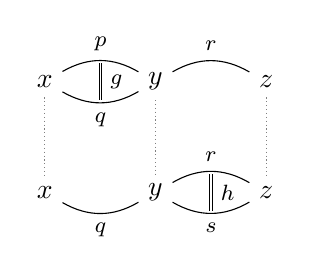
\begin{tikzpicture}[node distance=4em, baseline=(basenode.base)]
        \node[] (x1) {$x$};
        \node[right of=x1] (y1) {$y$};
        \node[right of=y1] (z1) {$z$};
        \node[below of=x1] (x2) {$x$};
        \node[right of=x2] (y2) {$y$};
        \node[right of=y2] (z2) {$z$};
        \draw[bend left] (x1) to node[above] (p) {\footnotesize$p$} (y1);
        \draw[bend right] (x1) to  node[below] (q1) {\footnotesize$q$} (y1);
        \draw[bend left] (y1) to node[above] (r1) {\footnotesize$r$} (z1);
        \draw[bend left] (y2) to node[above] (r2) {\footnotesize$r$} (z2);
        \draw[bend right] (y2) to  node[below] (s) {\footnotesize$s$} (z2);
        \draw[bend right] (x2) to node[below] (q2) {\footnotesize$q$} (y2);
        \draw[double, shorten >=.1em, shorten <=.1em] (p) to node[right] {\footnotesize$g$} (q1);
        \draw[double, shorten >=.1em, shorten <=.1em] (r2) to node[right] {\footnotesize$h$} (s);
        \draw[gray,densely dotted] (x1) to node (basenode){} (x2) (y1) to (y2) (z1) to (z2);
      \end{tikzpicture}%
      =%
      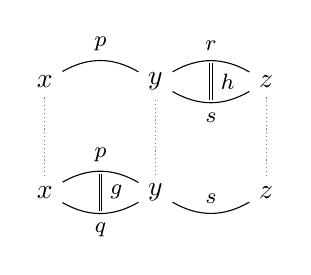
\begin{tikzpicture}[node distance=4em, baseline=(basenode.base)]
        \node[] (x1) {$x$};
        \node[right of=x1] (y1) {$y$};
        \node[right of=y1] (z1) {$z$};
        \node[below of=x1] (x2) {$x$};
        \node[right of=x2] (y2) {$y$};
        \node[right of=y2] (z2) {$z$};
        \draw[bend left] (x2) to node[above] (p) {\footnotesize$p$} (y2);
        \draw[bend right] (x2) to  node[below] (q1) {\footnotesize$q$} (y2);
        \draw[bend right] (y2) to node[above] (r1) {\footnotesize$s$} (z2);
        \draw[bend left] (y1) to node[above] (r2) {\footnotesize$r$} (z1);
        \draw[bend right] (y1) to  node[below] (s) {\footnotesize$s$} (z1);
        \draw[bend left] (x1) to node[above] (p2) {\footnotesize$p$} (y1);
        \draw[double, shorten >=.1em, shorten <=.1em] (p) to node[right] {\footnotesize$g$} (q1);
        \draw[double, shorten >=.1em, shorten <=.1em] (r2) to node[right] {\footnotesize$h$} (s);
        \draw[gray,densely dotted] (x1) to node (basenode){} (x2) (y1) to (y2) (z1) to (z2);
      \end{tikzpicture}%
    \end{sidecaption}
  \end{figure}%
  %
  One prove such a result by induction on $h$. Indeed, when
  $h\jdeq \refl r$, then both sides of the equation reduces through
  path algebra to $\ap {r\cdot\blank} (g)$. Now we are interested in
  this result when $x,y,z$ are all definitionally $a$, and $p,q,r,s$
  are all definitionally $\refl a$. In that case, one has that
  $\ap {\refl a\cdot \blank}$ and $\ap {\blank\cdot\refl a}$ both act
  trivially, and the equation becomes: $h\cdot g = g \cdot h$.

  One still has to prove that the function $\loopspace$ is an inverse
  for $\BB$. Given an abelian group $G$, the proof
  of~\cref{lemma:universal-cover-simply-connected} gives an
  equivalence between $\B\loopspace {(\BB G)}$ and the connected
  component of $\id_{\BG_\div}$ in $\BG_\div=\BG_\div$. By
  definition, this is the classifying type of $\grpcenter(G)$. Being
  abelian, $G$ is isomorphic to its center
  (\cref{def:abelian-groups}), and so it yields an element of
  $\loopspace {(\BB G)} =_{\typegroup} G$. %
  \marginnote[-1.5\baselineskip]{%
    If $X \ptdweq Y$ denote the type of pointed equivalences between
    pointed types $X,Y:\UUp$, then the univalence axiom implies that
    there is an equivalence
    \begin{displaymath}
      (X=Y) \weq (X \ptdweq Y).
    \end{displaymath}%
  }%
  Conversely, take a pointed simply connected $2$-type $(A,a)$. One
  wants to prove $\BB (\loopspace {(A,a)}) \weq_\ast (A,a)$. One
  should first notice that, because $\loopspace (A,a)$ is an abelian
  group,
  \begin{fullwidth}
  \begin{equation}
    \label{eq:loopspace-A-abelian}%
    {\B\loopspace \left( \BB (\loopspace {(A,a)}) \right)}
    \weq \conncomp{((a=a)=(a=a))}{\refl{a=a}} \weq (a=a,\refl a).
  \end{equation}
\end{fullwidth}
  This equivalence maps a path
  \begin{displaymath}
    (p,!):(a=a,\settrunc{\refl{a=a}})=(a=a,\settrunc{\refl{a=a}})
  \end{displaymath}
  to the evaluation $p(\refl a): a=a$.

  %% OLD MATERIAL, can still be useful.
  %%
  % We will now provide
  % \begin{displaymath}
  %   \Phi : \BB {(\loopspace {(A,a)})} \ptdto (A,a)
  % \end{displaymath}
  % such that $\loopspace(\Phi)$ is the previous equivalence.
  % To be able to
  % express $\Phi$, we need a small gadget about truncations of
  % function
  % types: for types $X,Y:\UU$, given an element
  % $f_0:\setTrunc{X\to Y}$, one constructs a map
  % $\lceil f_0 \rceil : \setTrunc X \to \setTrunc Y$; the type of
  % $\lceil f_0 \rceil$ being a set, one might as well suppose that
  % $f_0 \jdeq \settrunc f$ for some $f:X\to Y$; then we set
  % $\lceil f_0 \rceil (\settrunc x) = \settrunc{f(x)}$, which
  % suffices
  % in order to define $\lceil f_0 \rceil$ entirely because its
  % codomain
  % $\setTrunc Y$ is a set. If we assume the axiom of
  % choice\footnote{What is the status of AC in this book??}, then
  % $\lceil \blank \rceil$ is injective when $Y$ is a set.
  %%
  We will now define a pointed map
  $\Phi : (A,a) \ptdto \BB (\loopspace {(A,a)})$, and prove
  subsequently that this is an equivalence. Let $T : A \to \UU$ be the
  type family define by
  \begin{displaymath}
    T(a') \defequi \sum_{\alpha:\setTrunc{(a=a)\weq(a=a')}}
    \prod_{p:a=a'}\alpha=\settrunc {p\cdot\blank}
  \end{displaymath}
  We claim that $T(a')$ is contractible for all $a':A$. By
  connectedness of $A$, it is equivalent to showing that $T(a)$ is
  contractible. However
  \begin{align*}
    T(a)
    &\jdeq \sum_{\alpha:\setTrunc{(a=a)\weq(a=a)}}\prod_{p:a=a}
      \alpha = \settrunc {p\cdot \blank}
    \\
    &\weq \sum_{\alpha:\setTrunc{(a=a)\weq(a=a)}} \alpha = \settrunc{\id_{a=a}}
    \\
    &\weq 1
  \end{align*}
  Let then $\Phi (a')$ be the element
  $(a=a', \kappa_{a'}):\univcover \UU {a=a}$ where $\kappa_{a'}$ is
  the first projection of the center of contraction of $T(a')$. In
  particular, following the chain of equivalences above, $\Phi(a)$ is
  defined as $(a=a, \settrunc{\refl {a=a}})$, hence $\Phi(a)$ is
  trivially pointed by a reflexivity path. To verify that $\Phi$, thus
  defined, is an equivalence, one can use connectedness of
  $\BB(\loopspace (A,a))$ and only check that
  $\inv\Phi(a=a,\settrunc{\refl {a=a}})$ is contractible. However,
  \begin{displaymath}
    \inv\Phi(a=a,\settrunc{\refl {a=a}}) \simeq \sum_{a':A}
    \sum_{\varphi : (a=a) \weq (a=a')}\settrunc{\varphi} = \kappa_{a'}.
  \end{displaymath}
  For an element $a':A$ together with $\varphi: (a=a) \weq (a=a')$
  such that the proposition $\settrunc \varphi = \kappa_{a'}$ holds, a
  path between $(a,\id_{a=a},!)$ and $(a',\varphi,!)$ consists of a
  path $p:a=a'$ and a path $q:(x\mapsto p x) = \varphi$. We have a
  good candidate for $p$, namely $p\defequi \varphi(\refl
  a):a=a'$. However we don't have quite $q$ yet. Consider, for any
  $a':A$, the function
  \begin{fullwidth}
    \begin{displaymath}
      \ev_{\refl a}^{a'} :
      \left(
        (a=a, \settrunc{\refl{a=a}} ) =
        (a=a', \kappa_{a'} )
      \right)
      \to (a=a'),\quad (\psi,!) \mapsto \psi(\refl a)
    \end{displaymath}
  \end{fullwidth}
  Note that $\ev_{\refl a}^{a}$ is precisely the equivalence
  $\B\loopspace{(\BB\loopspace(A,a))}_\div \weq (a=a)$ described
  in~\cref{eq:loopspace-A-abelian}. Hence, by connectedness of $A$,
  one gets that the proposition $\isEq(\ev_{\refl a}^{a'})$ holds for
  all $a':A$. In particular, because the propositions
  $\settrunc \varphi = \kappa_{a'}$ and
  $\settrunc {p\cdot\blank} = \kappa_{a'}$ holds, one gets elements
  $(\varphi,!)$ and $(x\mapsto px,!)$ in the domain of
  $\ev_{\refl a}^{a'}$. Their image $\ev_{\refl a}^{a'}(\varphi,!)$
  and $\ev_{\refl a}^{a'}(x\mapsto px,!)$ are both equal to $p$, which
  provides a path $(x\mapsto px,!)=(\varphi,!)$ in the domain. The
  first component is the path $q:(x\mapsto px) = \varphi$ that we
  wanted.
\end{proof}


\section{$G$-sets vs $\abstr(G)$-sets}
\label{sec:Gsetsabstrconcr}
\marginnote{Recall from \cref{def:abstrGtorsors} that the type of $\abstr(G)$-set is
  $$Set_{\abstr(G)}^\abstr\defequi \sum_{\mathcal X:\Set}\Hom_\abstr({\abstr(G)},\abstr(\Sigma_{\mathcal X})).$$}

Given a group $G$ it should by now come as no surprise that the type of $G$-sets is equivalent to the type of $\abstr(G)$-sets.
According to \cref{lem:homomabstrconcr}
$$\abstr:\Hom(G,\Sigma_{\mathcal X})\to\Hom^\abstr(\abstr(G),\abstr(\Sigma_{\mathcal X}))$$
is an equivalence, where the group $\Sigma_{\mathcal X}$ (as a pointed connected groupoid) is the component of the groupoid $\Set$, pointed at $\mathcal X$.  The component information is moot since we're talking about pointed maps from $\BG$ and we see that $\Hom(G,\Sigma_{\mathcal X})$ is equivalent to $\sum_{F:\BG_\div\to\Set}(\mathcal X=F(\shape_G))$.  Finally,
$$\mathrm{pr}:\sum_{\mathcal X}\sum_{F:\BG_\div\to\Set}(\mathcal X=F(\shape_G))\we
(\BG_\div\to\Set),\quad \mathrm{pr}(\mathcal X,F,p)\defequi F
$$
is an equivalence (since $\sum_{\mathcal X}(\mathcal X=F(\shape_G))$ is contractible).
Backtracking these equivalences we see that we have established
\begin{lemma}
  \label{lem:actionsconcreteandabstract}
  Let $G$ be a group.  Then the map
  $$\ev_{\shape_G}:\GSet\to\Set^\abstr_{\abstr(G)},\qquad \ev_{\shape_G}(X)\defequi(X(\shape_G),a_X)
$$
is an equivalence, where the homomorphism $a_X:\Hom^\abstr(\abstr(G), \abstr(\Sigma_{X(\shape_G)}))$ is given by transport $X:\USym G\defequi(\shape_G=\shape_G)\to (X(\shape_G)=X(\shape_G))$.
\end{lemma}
If $X$ is a $G$-set, $g:\USym G$ and $x:X(\shape_G)$, we seek forgiveness for writing $g\cdot x:X(\shape_G)$ instead of $\cast(a_X(g))(x)$.\footnote{and I ask forgiveness for strongly disliking the use of ``$\cast$'' as a name for some tacitly understood map!}

\begin{example}
  \label{ex:abstrandconj}
  Let $H$ and $G$ be groups.  Recall that the set of homomorphisms from $H$ to $G$ is a $G$-set in a natural way:
$$\Hom(H,G):\BG\to\Set,\quad \Hom(H,G)(y)\defequi \sum_{F:\BH_\div\to \BG_\div}(y=F(\shape_H)).$$

What abstract $\abstr(G)$-set does this correspond to?
In particular, under the equivalence $\abstr:\Hom(H,G)\to\Hom^\abstr(\abstr(H),\abstr(G))$, what is the corresponding action of $\abstr(G)$ on the abstract homomorphisms?

The answer is that $g:\USym G$ acts on $\Hom^\abstr(\abstr(H),\abstr(G))$ by postcomposing with conjugation $c^g$ by $g$ as defined in \cref{ex:conjhomo}.

Let us spell this out in some detail:
If $(F,p):\Hom(H,G)(\shape_G)\defequi
 \sum_{F:\BH_\div\to \BG_\div}(\shape_G=F(\shape_H))$ and $g:\USym G$, then $g\cdot(F,p)\defequi(F,p\,g^{-1})$.  If we show that the action of $g$ sends $\abstr(F,p)$ to $c^g\circ\abstr(F,p)$ we are done.

Recall that $\abstr(F,p)$ consists of the composite
$$\xymatrix{\USym H\ar[r]^-{F^=}&(F(\shape_H)=F(\shape_G))\ar[rr]^-{t\mapsto p^{-1}t\,p}&&\USym G},$$
(\ie $\abstr(F,p)$ applied to $q:\USym H $ is  $p^{-1}F^=(q)\,p$)  together with the proof that this is an abstract group homomorphism.
We see that $\abstr(F,p\,g^{-1})$ is given by conjugation:
$q\mapsto(p\,g^{-1})^{-1}F^=(q)\,(p\,g^{-1})=g\,(p^{-1}F^=(q)\,p)\,g^{-1}$, or in other words $c^g\circ\abstr(F,p)$.
\end{example}
For reference we list the conclusion of this example as a lemma:
\begin{lemma}\label{lem:abstrandconj}
  If $H$ and $G$ are groups, then the equivalence of \cref{lem:actionsconcreteandabstract} sends the $G$-set $\Hom(H,G)$ to the $\abstr(G)$-set $\Hom^\abstr(\abstr(H),\abstr(G))$ with action given by postcomposing with conjugation by elements of $\abstr(G)$.
\end{lemma}

If $f:\Hom(G,G')$ is a homomorphism, then precomposition with $\Bf:\BG\to \BG'$ defines a map $$f^*:(G'\text{-}\Set)\to(G\text{-}\Set).$$
\marginnote{Recall that \cref{lem:eq-mono-cover} told us that $f$ is an epimorphism precisely when $\USym f$ is a surjection.}
We will have the occasion to use the following result which essentially says that if $f:\Hom(G,G')$ is an epimorphism, then $f^*$ embeds the type of $G'$-sets as some of the components of the type of $G$-sets.
\begin{lemma}
  \label{lem:epifullyfaithful}
  Let $G$ and $G'$ be groups and let $f:\Hom(G,G')$ be an epimorphism.
  Then the map $f^*:(G'\text{-}\Set)\to(G\text{-}\Set)$ (induced by precomposition with $\Bf:\BG\to \BG'$) is ``fully faithful'' in the sense that if $X,Y$ are $G'$-sets, then
$$f^*:(X=Y)\to(f^*X=f^*Y)
$$
is an equivalence.
\end{lemma}
\begin{proof}
  Evaluation at $\shape_G$  yields an injective map
$$\mathrm{ev}_{\shape_G}:(f^*X=f^*Y)\to(X(f(\shape_G)=Y(f(\shape_G)))$$ and the composite
$$\mathrm{ev}_{\shape_G}f^*=\mathrm{ev}_{f(\shape_G)}:(X=Y)\to(X(f(\shape_G)=Y(f(\shape_G)))$$
 is the likewise injective, so $f^*:(X=Y)\to(f^*X=f^*Y)$ is injective.

For surjectivity, let $F':f^*X=f^*Y$ and write, for typographical convenience, $a:X(f(\shape_G)=Y(f(\shape_G))$ for $\mathrm{ev}_{\shape_G}F'\defequi F'_{\shape_G}$.
By the equivalence between $G$-sets and $\abstr(G)$-sets, $F'$ is uniquely pinned down by $a$ and the requirement that for all $g'=f(g)$ with $g:\USym G$ the diagram
$$\xymatrix{X(f(\shape_G))\ar@{=}[r]^{X({g'})}\ar@{=}[d]_{a}&
  X(f(\shape_G))\ar@{=}[d]_{a}\\
  Y(f(\shape_G))\ar@{=}[r]^{Y({g'})}&Y(f(\shape_G))}
$$
commutes.  Likewise, (using transport along the identity $p_f:\shape_{G'}=f(\shape_G)$) an $F:X=Y$ in the preimage of $a$ is pinned down by the commutativity of the same diagram, but with $g':f(\shape_G)=f(\shape_G)$ arbitrary (an a priori more severe requirement, again reflecting injectivity).   However, when $f:\USym G\to\USym {G'}$ is surjective these requirements coincide, showing that $f^*$ is an equivalence.


% Fix for the moment an  $a:X(f(\shape_G)=Y(f(\shape_G))$

% Now, by transport along the identity $p_f:\shape_{G'}=f(\shape_G)$ and the equivalence between $G'$-sets and $\abstr(G')$-sets, an identity $F':X=Y$ of $G'$-sets is uniquely pinned down by an identity $F'_{f(\shape_G)}:X(f(\shape_G)=Y(f(\shape_G))$ together with the proposition that for all $g':f(\shape_G)=f(\shape_G)$ the diagram $$\xymatrix{X(f(\shape_G))\ar@{=}[r]^{X_{g'}}\ar@{=}[d]_{F'_{f(\shape_G)}}&
%   X(f(\shape_G))\ar@{=}[d]_{F'_{f(\shape_G)}}\\
%   Y(f(\shape_G))\ar@{=}[r]^{Y_{g'}}&Y(f(\shape_G))}
% $$
% commutes.  Likewise, an identity $F:f^*X=f^*Y$ is given by exactly the same data, except that the diagram is only required to commute for $g'=f(g)$ for all $g:\USym G$.  But when $f:\USym G\to\USym {G'}$ these requirements coincide.


% ; $F:X=Y$ is in the preimage of $a:X(f(\shape_G)=Y(f(\shape_G))$ if and only if $a=F_{f(\shape_G)}$ and for all $g':f(\shape_G)=f(\shape_G)$ the diagram
% $$\xymatrix{X(f(\shape_G))\ar@{=}[r]^{X_{g'}}\ar@{=}[d]_{F_{f(\shape_G)}}&
%   X(f(\shape_G))\ar@{=}[d]_{F_{f(\shape_G)}}\\
%   Y(f(\shape_G))\ar@{=}[r]^{Y_{g'}}&Y(f(\shape_G))}
% $$
% commutes.  However, since $f$ is surjective there is a $g:\USym G$ so that $g'=f(g)$.  Therefore, anything in $f^*X=f^*Y$ which is in the preimage of $a$ is in the image of $f^*:X=Y$ and we have shown that $f^*$ is also a surjection.
\end{proof}



\section{Sums of groups}
\label{sec:coprod}
We have seen how the group of integers $\ZZ=(S^1,\base)$ synthesizes the notion of one symmetry with no relations: every symmetry in the circle is of the form $\Sloop^n$ for some unique $n$.  Also, given any group $G=\aut_A(a)$, the set $a=a$ of symmetries of $a$ corresponds to the set of homomorphisms $\ZZ\to G$, \ie to pointed functions $(S^1,\base)\to_*(A,a)$ by evaluation at $\Sloop$.  What happens if we want to study more than one symmetry at the time?

For instance, is there a group $\ZZ\vee\ZZ$ so that for any group $G=\aut_A(a)$ a homomorphism $\ZZ\vee\ZZ\to G$ corresponds to {\bf two} symmetries of $a$?
At the very least, $\ZZ\vee\ZZ$ itself would have to have two symmetries and these two can't have any relation, since in a general group $G=\aut_A(a)$ there is a priori no telling what the relation between the symmetries of $a$ might be.
Now, \emph{one} symmetry is given by a pointed function $(S^1,\base)\to_*(A,a)$ and so a \emph{pair} of symmetries is given by a function $f:S^1+S^1\to A$ with the property that $f$ sends each of the base points of the circles to $a$.  But $S^1+S^1$ is not connected, and so not a group.  To fix this we take the clue from the requirement that both the base points were to be sent to a common base point and \emph{define} $S^1\vee S^1$ to be what we get from $S^1+S^1$ when we \emph{insert an identity} between the two basepoints.
\marginnote{$S^1\vee S^1$ if formed from $S^1+S^1$ by inserting an identity$$\xymatrix{\base\ar@(ul,dl)[]|{\Sloop}\ar@{.>}[rr]^{\text{identify!}}&&\base\ar@(ur,dr)[]|{\Sloop}}
  $$}

The amazing thing is that this works -- an enormous simplification of the classical construction of the ``free products'' or ``amalgamated sum'' of groups.  We need to show that the ``wedge'' $S^1\vee S^1$ is indeed a group, and this proof simultaneously unpacks the classical description.

We start by giving a definition of the wedge construction which is important for pointed types in general and then prove that the wedge of two groups is a group whose symmetries are arbitrary ``words'' in the original symmetries.

\begin{definition}
  \label{def:wedge}
  Let $(A_1,a_1)$ and $(A_2,a_2)$ be pointed types.  The \emph{wedge}\index{wedge of pointed types} is the pointed type $(A_1\vee A_2,a_{12})$ given as a higher inductive type by
  \begin{enumerate}
  \item functions $i_1:A_1\to A_1\vee A_2$ and $i_2:A_2\to A_1\vee A_2$
  \item an identity $g:i_1a_1=i_2a_2$.
  \end{enumerate}
We point this type at $a_{12}\defequi i_1a_1$.
  The function
$$i^g_2:(a_2=_{A_2}a_2)\to(a_{12}=_{A_1\vee A_2}a_{12})$$
is defined by $i^g_2(p)\defequi g^{-1}i_2(p)g$, whereas (for notational consistency only) we set $i_1^g\defequi i_1:(a_1=_{A_1}a_1)\to(a_{12}=_{A_1\vee A_2}a_{12})$.
Simplifying by writing $i:A_1+A_2\to A_1\vee A_2$ for the function given by $i_1$ and $i_2$ (with basepoints systematically left out of the notation),
the induction principle is
$$\prod_{C:(A_1\vee A_2)\to\UU}\sum_{s:\prod_{a:A_1+A_2}Ci(a)}
((s(a_1)=C(g^{-1})s(a_2))\,\to\,\prod_{x:(A_1\vee A_2)}C(x)).$$
\end{definition}

Unraveling the induction principle we see that if $B$ is a pointed type, then a  pointed function $f:A_1\vee A_2\to_* B$ is given by providing pointed functions $f_1:A_1\to_* B$ and $f_2:A_2\to_* B$  -- the identity $f_1(a_1)=f_2(a_2)$ which seems to be missing is provided by the requirement of the functions being pointed.  For the record
\begin{lemma}
  \label{lem:univvee}
  If $B$ is a pointed type, then the function
  $$i^*:(A_1\vee A_2\to_*B)\to(A_1\to_*B)\times(A_2\to_*B),\qquad i^*(f)=(fi_1,fi_2)
$$
is an equivalence.
\end{lemma}



To the right you see a picture of $i_2^g(p)$: \marginnote{$$
\xy (-20,20)*+{};(-20,20)*+{}
**\crv{(15,20)&(18,20)&(-10,35)&(10,45)&(25,30)&(20,19)&(0,20)}
%?>*\dir{>}
?(0)*{} *!LD!/^-20pt/{i_1A_1}
?(.45)*{} *!LD!/^2pt/{>}
?(.95)*{} *!LD!/^-15pt/{g^{-1}}
?(.03)*{} *!LD!/^-5pt/{g}
?(.55)*{} *!LD!/^-7pt/{i_2p}
?(.65)*{} *!LD!/^-30pt/{i_2A_2}
?(.87)*{} *!LD!/^-12pt/{i_2a_2}
?(.86)*{} *!LD!/^-2pt/{\bullet}
?(1)*{} *!LD!/^-2pt/{\bullet}
?(1)*{} *!LD!/^-12pt/{a_{12}}
\endxy
$$}it is the symmetry of the base point $a_{12}\defequi i_1a_1$ you get by \emph{first} moving to $i_2a_2$ with $g$, \emph{then} travel around with $p$ ($i_2p$, really) and finally go home to the basepoint with the inverse of $g$.

\marginnote{The idea is that an identity in $a_{12}=x$ can be factored into a string of identities, each lying solely in $A_1$ or in $A_2$.  We define a family of sets consisting of exactly such strings of identities --  it is a set since $A_1$ and $A_2$ are groupoids -- and prove that it is equivalent to the family $P(x)\defequi(a_{12}=_{A_1\vee A_2}x)$ which consequently must be a family of sets.
We need to be able to determine whether a symmetry is reflexivity or not, but once we know that, the symmetries of the base point in the wedge are then given by ``words $p_0p_1\dots p_n$'' where the $p_j$ alternate between being symmetries in the first or the second group, and none of the $p_j$ for positive $j$ are allowed to be reflexivity.  Note that there order of the $p_j$s is not negotiable: if I shuffle them I get a new symmetry.}


\begin{definition}
  \label{def:sumofgroup}
  If $G_1=\aut_{A_1}(a_1)$ and $G_2=\aut_{A_2}(a_2)$ are groups, then their \emph{sum}\index{sum of groups} is defined as
  $$G_1\vee G_2\defequi \aut_{A_1\vee A_2}(a_{12}).$$
  The homomorphisms $i_1:G_1\to G_1\vee G_2$ and $i_2:G_2\to G_1\vee G_2$ induced from the structure maps  $i_1:A_1\to A_1\vee A_2$ and  $i_2:A_2\to A_1\vee A_2$ are also referred to as \emph{structure maps}.
\end{definition}
\begin{lemma}
  \label{lem:sumofgroupsISsum} If $G_1$, $G_2$ and $G$ are groups, then the function
  $$\Hom(G_1\vee G_2,G)\to\Hom(G_1,G)\times\Hom(G_2,G)$$
given by restriction along the structure maps is an equivalence.
\end{lemma}
\begin{proof}
  This is a special case of \cref{lem:univvee}.
\end{proof}
Specializing further, we return to our initial motivation and see that mapping out of a wedge of two circles \emph{exactly} captures the information of two independent symmetries:
\begin{corollary}
  \label{cor:ZplusZuniv}
  If $G$ is a group, then the functions
  $$\Hom(\ZZ\vee\ZZ,G)\to \Hom(\ZZ,G)\times\Hom(\ZZ,G)\simeq \USym G\times \USym G$$
  is an equivalence.
\end{corollary}
\begin{xca}
This leads to the following characterization of abelian groups formulated purely in terms of pointed connected groupoids (no reference to the identity types).
  \label{xca:whatAREabeliangroups}
  A group $G$ is abelian if and only if the canonical map

  \marginnote{$$\xymatrix{G\vee G\ar[r]^+\ar[d]_{\text{inclusion}}&G\\
      G\times G\ar@{.>}[ur]}$$}
$$+:G\vee G\to G$$
(given via \cref{lem:sumofgroupsISsum} by $\id_G:G\to G$) extends over the inclusion
$$i:G\vee G\to G\times G$$
(given by the inclusions $\mathrm{in}_1,\mathrm{in}_2:G\to G\times G$).\footnote{I haven't written out a formalization myself}

As a cute aside, one can see that the required map $\BG\times\BG\to_*\BG$ actually doesn't need to be pointed:
factoring $+:\BG\vee\BG\to_*\BG$ over $i:\BG\vee\BG\to_*\BG\times\BG$
-- even in an unpointed way -- kills all ``commutators''
$ghg^{-1}h^{-1}:\USym(G\vee G)$.
\end{xca}

We end the section by proving that wedges of decidable groups are decidable groups and that they can be given the classical description in terms of words.


\begin{lemma}
  \label{lem:wedgeofgpoidisgpoid}
  Let $G_1\defequi\aut_{A_1}(a_1)$ and $G_2\defequi\aut_{A_2}(a_2)$ be decidable groups, then the wedge sum $G_1\vee G_2\defequi\aut_{A_1\vee A_2}(a_{12})$ is a decidable group.

Let $C_1$ be the set of strings $(p_0,n,p_1,\dots,p_n)$ with $n:\NN$ and, for $0\leq j\leq n$
\begin{itemize}
\item $p_{j}:\USym G_1%\defequi (a_1=a_1)
  $  for even $j$
\item $p_{j}:\USym G_2%\defequi (a_2=a_2)
  $ for odd $j$ and
\item $p_j$ is not reflexivity for $j$ positive
\end{itemize}
(the last requirement makes sense and is a proposition since our groups are decidable).

  Then the function given by composition in $\USym G_{12}\defequi(a_{12}=a_{12})$
  $$\beta:C_1\to\USym G_{12}%\defequi(a_{12}=a_{12})
  ,\qquad\beta(p_0,n,p_1,\dots p_n)\defequi i_1^gp_0i_2^gp_1i_1^gp_2\dots i_?^gp_n$$
(where $i_?^gp_n$  is $i_1^gp_n$ or $i_2^gp_n$ according to whether $n$ is even or odd) is an equivalence.
\end{lemma}
\begin{proof}
  That the wedge is connected follows by transitivity of identifications,
  if necessary passing through the identification $g:i_1a_1=i_2a_2$ in the wedge.

We must prove that the wedge is a groupoid, \ie that all identity types are sets, which we do by giving an explicit description of the universal \covering.

 We use the notation of \cref{def:wedge} freely, and for ease of notation, let $a_{2k+i}\defequi a_i$ and $i_{2k+i}^g\defequi i_i^g$ for $i=1,2$, $k:\NN$.
Define families of sets
$$C_i:A_i\to\Set,\qquad i=1,2$$
by
$$
C_i(x)\defequi(a_i=_{A_i}x)\times
\sum_{n:\NN}\prod_{1\leq k\leq n}\sum_{p_k:a_{i+k}= a_{i+k}}(p_k\neq\refl {a_{i+k}})
$$
when $x:A_i$.  Note that $p_k\neq\refl{a_{i+k}}$  is a proposition; we leave it out when naming elements. Hence, an element in $C_1(a)$ is a tuple
$(p_0,n,p_1,\dots,p_n)$ where $p_0:a_1=_{A_1}a$, $p_1:a_2=_{A_2}a_2$, $p_2:a_1=_{A_1}a_1$, and so on -- alternating between symmetries of $a_1$ and $a_2$, and where $p_0$ is the only identity allowed to be $\refl{}$. Define $C_{12}:C_1(a_1)\to C_2(a_2)$ by
$$C_{12}(p_0,n,p_1\dots,p_n)=
\begin{cases}
  (\refl{a_2}0,)&\text{ if }p_0=\refl{a_1}, n=0,\\
  (p_1,n-1,p_2\dots,p_n)& \text{ if }p_0=\refl{a_1},n\neq0,\\
  (\refl{a_2},n+1,p_0,\dots,p_n)& \text{ if }p_0\neq\refl{a_1}.
\end{cases}
$$
It is perhaps instructive to see a table of the values $C_{12}(p_0,n,p_1,\dots,p_n)$ for $n<3$:
\begin{center}
  \begin{tabular}{r|c cc}
    &$(p_0,0)$&$(p_0,1,p_1)$&$(p_0,2,p_1,p_2)$\\
    \hline
    $p_0=\refl{a_1}$&$(\refl{a_2},0)$&$(p_1,0)$&$(p_1,1,p_2)$\\
    $p_0\neq\refl{a_1}$&$(\refl{a_2},1,p_0)$&$(\refl{a_2},2,p_0,p_1)$&$(\refl{a_2},3,p_0,p_1,p_2)$
  \end{tabular}
\end{center}
Since $C_{12}$ is an equivalence, the triple $(C_1,C_2,C_{12})$ defines a family
$$C:A_1\vee A_2\to\Set.$$
In particular, $C(a_{12})\defequi C_1(a_1)$.
For $x:A_1$ we let $i^C_1:C_1(x)\to C(i_1(x))$ be the induced equivalence, and likewise for $i^C_2$.
We will show that $C$ is equivalent to $P\defequi \pathsp{a_{12}}$, where $P(x)\defequi(a_{12}=x)$, and so that the identity types in the wedge are equal to the sets provided by $C$.

One direction is by transport in $C$; more precisely,
$$\alpha:\prod_{x:A_1\vee A_2}(P(x)\to C(x))$$ is given by transport with $\alpha(a_{12})(\refl{a_{12}})\defequi(\refl{a_{1}},0):C(a_{12})$.
The other way,
$$\beta:\prod_{x:A_1\vee A_2}(C(x)\to P(x))$$ is given by composing identities, using the glue $g$ to make their ends meet:
$$\beta(i_1a)(p_0,n,p_1,\dots,p_n)\defequi i_1(p_0)i_2^g(p_1)i_3^g(p_2) \dots i_{n+1}^g(p_n)$$
(here the definition $\dots i_3^g\defequi i_1^g\defequi i_1$ proves handy since we don't need to distinguish the odd and even cases)
and likewise
$$\beta(i_2a)(p_0,n,p_1,\dots,p_n)\defequi i_2(p_0)g\,i_1^g(p_1)i_2^g(p_2) \dots i_{n}^g(p_n)$$ and compatibility with the glue $C_{12}$ is clear since the composite $\refl{x}p$ is equal to $p$.

For notational convenience, we hide the $x$ in $\alpha(x)(p)$ and $\beta(x)(p)$ from now on.

That $\beta\alpha(p)=p$ follows by path induction: it is enough to prove it for $x=a_{12}$ and
$p\defequi\refl{a_{12}}$:
$$\beta\alpha(\refl{a_{12}})=\beta(\refl{a_1},0)=i_1^g\refl{a_1}=\refl{a_{12}}.$$

That $\alpha\beta(p_0,n,p_1\dots,p_n)=(p_0,n,p_1,\dots,p_n)$ follows by induction on $n$ and $p_0$.  For $n=0$ it is enough to consider  $x=a_{12}$ and $p_0=\refl{a_1}$, and then
$\alpha\beta(\refl{a_1},0)\defequi\alpha(\refl{a_{12}})\defequi(\refl{a_1},0)$.  In general, (for $n>0$)
\begin{align*}
  \alpha\beta(p_0,n,p_1\dots,p_n)
=&\trp[C]{i_1(p_0)i_2^g(p_1)i_1^g(p_2) \dots i_{n+1}^g(p_n)}(\refl{a_1,0})\\
=&\trp[C]{i_1(p_0)}\dots\trp[C]{i_{n+1}^g(p_n)}(\refl{a_1,0}).
\end{align*}
  The induction step is as follows: let $0< k\leq n$, then
\begin{align*}
  &\trp[C]{i_k^gp_{k-1}}i^C_{k-1}(p_k,n-k-1,p_{k+1},\dots,p_n)\\
  =&\trp[C]{i_k^gp_{k-1}}i^C_k(\refl{a_{k-1}},n-k,p_k,\dots,p_n)\\
  =&i^C_k\trp[C_k]{p_{k-1}}(\refl{a_{k-1}},n-k,p_k,\dots,p_n)\\
  =&(p_{k-1},n-k,p_k,\dots,p_n).
\end{align*}
%((please see whether this makes sense to anybody but yvt))
\end{proof}

% Local Variables:
% fill-column: 144
% latex-block-names: ("lemma" "theorem" "remark" "definition" "corollary" "fact" "properties" "conjecture" "proof" "question" "proposition" "exercise")
% TeX-master: "book"
% End:
